\documentclass[a4paper,12pt]{article}
\usepackage[english]{babel}
\usepackage{graphicx}
\graphicspath{ {figures/} }
\usepackage{array}
\usepackage[colorinlistoftodos]{todonotes}
\usepackage[a4paper,%bindingoffset=0.2in,%
            left=2.5cm,right=2.5cm,top=3cm,bottom=3cm%footskip=1.5pt
            ]{geometry} %margins
\usepackage{placeins}
\usepackage{amsmath,amsfonts,amssymb}
\newcommand{\underwrite}[3][]{% \underwrite[<thickness>]{<numerator>}{<denominator>}
  \genfrac{}{}{#1}{}{\textstyle #2}{\scriptstyle #3}
}
\usepackage{titlesec}

\setcounter{secnumdepth}{4}
\setcounter{tocdepth}{4}
\usepackage{hyperref}
\usepackage{subcaption}
\usepackage{caption}
\usepackage{float}
\usepackage{color}
\usepackage{listings}
\usepackage{parskip}
\usepackage[framed,numbered,autolinebreaks, useliterate]{mcode}
\lstset{language=Matlab}%
\renewcommand{\familydefault}{\sfdefault}
\numberwithin{equation}{section}

\begin{document}

\begin{titlepage}

\newcommand{\HRule}{\rule{\linewidth}{0.5mm}} % Defines a new command for the horizontal lines, change thickness here

\center % Center everything on the page
 
%----------------------------------------------------------------------------------------
%	HEADING SECTIONS
%----------------------------------------------------------------------------------------

\begin{figure}[h]
    
\includegraphics[scale=0.5]{logos_bruface.pdf}\\[1cm] 
\end{figure}

%\textsc{\LARGE Brussels faculty of Engineering}\\[1.5cm] % Name of your university/college
\vspace{1cm}
%\textsc{\Large MEMO-H503 }\\[0.5cm] % Major heading such as course name
\vspace{0.5cm}
\textsc{\large Master Thesis in Electrical Engineering}\\[0.5cm] % Minor heading such as course
%title
\textsc{\large Romaric Noumo}\\[0.5cm]


\HRule \\[0.5cm]
{ \huge \bfseries MISO data driven modelling of the temperature of a Building}\\[0.4cm] % Title of your document
\HRule \\[1.5cm]
 
%\hspace{-1.5cm}
%\begin{minipage}{1\textwidth}

%\begin{flushleft} \large
%\emph{Author:}\\
%Romaric\textsc{ Noumo}  \\
%\end{flushleft}
%\end{minipage}

%\hspace{1cm}
\begin{minipage}{1\textwidth}
\begin{flushright} \large
\emph{Master	thesis	submitted	under	the	supervision	of:} \\
Prof. John \textsc{Lataire} \\
\vspace{1cm}
\emph{The	co-supervision	of:} \\
Prof. Valéry-Ann\textsc{ Jacobs} \\
\vspace{1cm}
\emph{In	order	to	be	awarded the	
Master’s	Degree	in Electrical Engineering	} \\
\end{flushright}
\end{minipage}\\[2cm]




\vfill
{\large 2021-2022}\\[2cm] % Date, change the \today to a set date if you want to be precise

\end{titlepage}

%----------------------------------------------------------------------------------------
%\clearpage
\newpage

\begin{abstract}

The purpose of this thesis was to perform data-driven modelling to derive a MISO model of the the indoor operative temperature of a case-study building.The data was obtained from the Building simulator EnergyPlus. The inputs to the system being studied were the power of the heater in the building and the outdoor dry bulb temperature from weather files.The model obtained is to be used later on  for optimizing control strategies.

In the literature current system identification approaches  being used are model reduction and Machine learning techniques.In this thesis model reduction techniques were used, in particular Linear Least square Techniques.Intuitively one could say that the response of the system to the the outdoor dry bulb temperature is a slower process than the response to the heater.This is why different denominators for  the transfer functions of the two inputs were obtained. 

Using the data obtained from EnergyPlus, Linearity was first assessed and then for each input a a non-parametric model was obtained and then a first-order parametric model was then obtained using the non-parametric model. The heater power is a controllable input, as such, we can design it's input signal and  a multisine signal was chosen  as excitation signal to  determine the model from heater to indoor temperature.As for the dry bulb temperature,it is an uncontrollable input that is an arbitrary signal.It was  obtained from a weather file and was used as excitation signal to determine the model from dry bulb temperature to indoor temperature. 

Using different denominators for the transfer function yielded models with good prediction accuracy which described well the data.In addition, the models obtained were of low complexity making simulations fast and the implementation  of control strategies simpler.
\end{abstract}

\newpage

\tableofcontents
\newpage
%\listoffigures
\newpage

\setlength{\parindent}{1em}

\section{Introduction}
Healthy habitats aims at creating healthy indoor environment in our Living and working spaces.The global concern today is to reduce energy consumption.Health and comfort of the occupants should also be addressed.The smart healthy habitats concept is to achieve this two goals that is energy efficiency of the habitat and health and comfort of the residents.This is made possible with systems like Smart ventilation for healthy indoor air, external sun protection for visual and thermal comfort and free and natural cooling.The smart nature of these systems is due to large amount of sensors that learn about the condition of the building and actuators that acts upon it to create an optimal condition.The control actions of the users  not always being effective for the comfort control and energy efficient needs, the efficient control actions are created by control algorithms based on a model of the building.All of these in an automated approach.The aim of this thesis will be the modelling of a building from a system perspective with controllable input as heating, uncontrollable input as weather condition more specifically the dry bulb outside temperature and output as indoor operative temperature that is the thermal behaviour of the building.  

The system model is obtained in a data-driven modelling approach which consists of identifying a mathematical relationship between the input and the output of a system with limited knowledge about the physical behaviour of the system and often called black-box models.The data used is obtained either by measurements or by simulation software.In this thesis the data was obtained through a simulation software.Several simulation tools of buildings and their envelopes are available.They allow for virtual prototyping of realistic buildings and provide simulated data from physical modelling (including building geometry, heat transfer, impact of the sun and wind, ...).The Building Energy Simulation (BES) software that was used is EnergyPlus, an open-source software developed and funded by the U.S. Department of Energy(DOE).A  single-room case-study building, equipped with a heater was set up in EnergyPlus.The two inputs were seperately applied to the case-study building and the output was retrieved.The input-output data is then used to build a model using system Identification techniques in Matlab.Then the model was validated.The validated model will then be used in a future study in Model Predictive Control(MPC) or in reinforcement learning types of control strategies to enable a smart healthy habitat.

Several thermal behaviour modelling of a building are available in the literature.



\newpage

\section{Heat transfer in Buildings}
Thermodynamics defines heat as diffuse and chaotic in contrast to energy transmitted as work which is purposeful and organized.Particle physics defines heat as the statistically distributed kinetic energy of atoms and free electrons.Heat is the least noble, most diffuse form of energy to which each nobler form degrades.The temperature reflects the quality of the heat.Higher temperatures require warming up, lower temperatures cooling down of a system. Heat cannot be
measured directly. It is sensed and because many material properties depend on it, indirectly quantifiable.The SI system advances two temperature scales, one empiric in degrees Celsius, °C,
with the symbol $\theta$, and one thermodynamic in degrees kelvin, $K$, with the symbol $T$.The three mechanisms of heat transfer are y conduction, convection and radiation.

Conduction refers to the heat exchanged when vibrating atoms collide and free electrons move.It intervenes in solids,liquid and gas.A medium is required between the two bodies and like all heat transfer mechanism the two bodies must have different temperatures.No movement is induced in conduction and always goes in the direction of lower temperatures.Convection happens as a result of motion in  fluids such as air or water wherein temperatures differences exist,included contact with colder or warmer solids.Depending on the cause of movement whether it is an external force, a difference in density or both we will distinguish forced, natural or mixed convection.Convection needs a medium.Radiation, finally, concerns the heat transferred due to the emission and absorption of electromagnetic waves by surfaces. At temperatures above 0 $K$, every surface emits. If two or more are at different temperatures, the result is heat exchange.Radiation does not need a medium.The derivation of the laws governing this heat transfer mechanism can been viewed in appendix.

Some of the heat transfer processes that can take place in a building are illustrated in fig\ref{fig:heattransfer1} which shows a room on an intermediate floor in a multi-storey building.These heat transfer processes are:
\begin{enumerate}
    \item conduction heat transfer through the building fabric elements, including the external
walls, roof, ceiling and floor slabs and internal partitions;
    \item solar radiation transmission and conduction through window glazing;
    \item infiltration of outdoor air and air from adjoining rooms;
    \item heat dissipation from the lighting, equipment, occupants and other materials inside the room; and
    \item heating or cooling  provided by the HVAC system.
\end{enumerate}

\begin{figure}[H]
    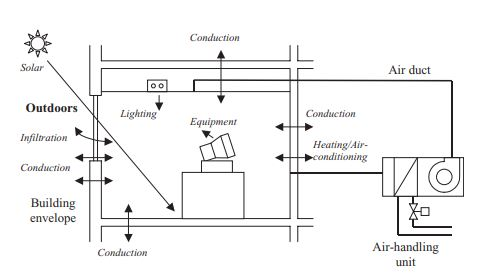
\includegraphics[scale=1.3]{heat_transfer.JPG}
    \centering
    \caption{Heat transfer processes involved in a building}
    \label{fig:heattransfer1}
\end{figure}

The conduction heat transfer through an opaque building fabric element, such as an external
wall as shown in Figure\ref{fig:heattransfer2}.This heat transfer is the effect of the convective heat that the surface at each side of the element is exchanging with the surrounding air and the radiant heat exchanges with other surfaces that the surface is exposed to. For an external wall or a roof, the radiant heat exchange at the external side includes the absorbed solar radiation.

\begin{figure}[H]
    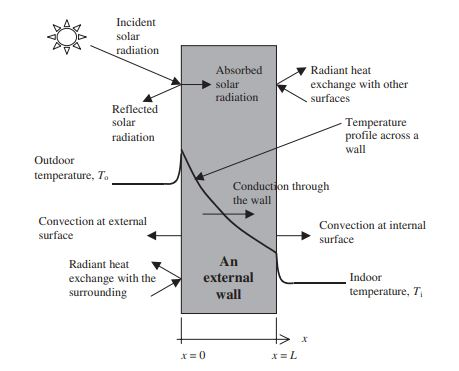
\includegraphics[scale=0.8]{heat_transfer2.JPG}
    \centering
    \caption{Heat transfer at an external wall}
    \label{fig:heattransfer2}
\end{figure}

The heat transfer through a window is shown in Figure\ref{fig:heattransfer3}.The window glass will transmit part of the incident solar radiation into the indoor space. While the solar radiation penetrates the glass pane, some of the energy will be absorbed by the glass, leading to an increase in the glass temperature, which, in turn, will cause heat to flow in both the indoor and the outdoor directions, first by conduction within the glass and then by convection and radiation at the surfaces at both sides.

\begin{figure}[H]
    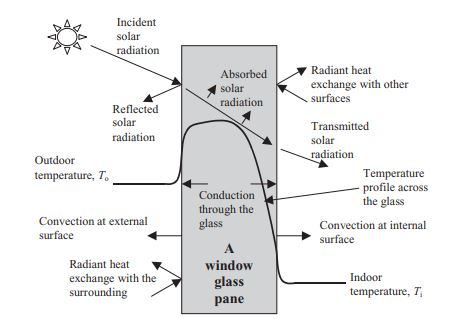
\includegraphics[scale=0.8]{heat_transfer3.JPG}
    \centering
    \caption{Heat transfer at a window glass pane}
    \label{fig:heattransfer3}
\end{figure}

Several models of heat transfer in a building are available.White box models are used by BES and are physically based models that rely on the understanding of the underlying processes to model and solve a set of heat transfer equations.Grey-box model uses both physical insights coupled with measurements data to complete the model.A popular grey-box model is the thermal network model, an electrical analogy of the dynamics of a building.Thermal resistance is modelled as resistors and
thermal capacitance as capacitors. The resulting model is a circuit where the temperature is used as the driving potential, and the flow through the circuit is the heat    flow.Fig\ref{fig:thermalmodel} shows the electrical circuit equivalent  of the thermal network model.


\begin{figure}[H]
    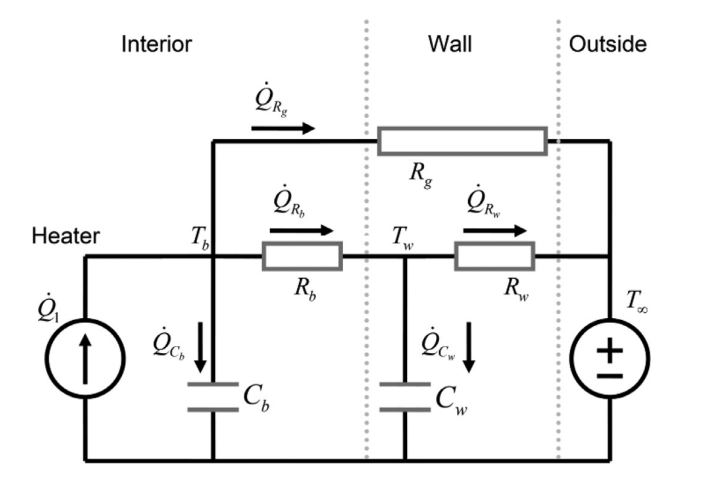
\includegraphics[scale=0.5]{thermal.JPG}
    \centering
    \caption{Electrical circuit equivalent  of the thermal network model}
    \label{fig:thermalmodel}
\end{figure}

\noindent
The model consists of two states $T_{b}$ and $T_{w}$, which correspond to the interior temperature of the building and the wall temperature respectively.Wall temperature is measured on the inner surface of the wall. For each state there is an associated capacitance,$C_{b}$ and $C_{w}$. These capacitances represent the building’s ability to store thermal energy in the interior and the building envelope, e.g.walls, floor and ceiling. The remaining three model components are resistances. $R_{b}$ represents the thermal resistance between the building interior and the wall. $R_{w}$ is the resistance to heat flow through the wall, i.e. between the state $T_{w}$ and the outside temperature. The third resistance $R_{g}$ represents the resistance to heat flow through the parts of the building envelope that are not included in the state $T_{w}$, such as windows and the door. The driving forces of the system are $\dot{Q}$ and $T_{\infty}$, where $\dot{Q}$ is a heat flow source, e.g. a heater and the outside temperature is modelled as a potential source $T_{\infty}$. Black-box models are the models we are aiming at obtaining in this thesis.

\newpage
\section{Building Description}
In this chapter the description of the building at study and to be set up in EnergyPlus will be given as well as a brief description of EnergyPlus with some of its features and parameters.

EnergyPlus is a freeware fully integrated building and HVAC simulation program  use to model both energy consumption for heating, cooling, ventilation, lighting and plug and process loads and water use in buildings.Some of the notable features and capabilities of EnergyPlus include:
\begin{itemize}
  \item Combined heat and mass transfer model that accounts for air movement between zones;
  \item Illuminance and glare calculations for reporting visual comfort and driving lighting controls.
  \item A large number of built-in HVAC and lighting control strategies and an extensible runtime scripting system for user-defined control.
\end{itemize}

\noindent
EnergyPlus uses a white-box model approach to predict the outputs based on specific inputs.Simulation was preferred to experimentation because it is much less expensive and less time consuming.The computation of the output is accurate provided the building description correctly done.Accuracy of the output requires to have all the properties of the building needed by the simulator which is not always easy to have.The simulation can be time consuming and is not suitable for real-time control and as such a black-box model which is less complex is preferred for prediction.Some of the parameters that were taken into account to obtain data for the system model estimation are:

\subsection{Weather conditions}
The weather conditions are the outdoor components that affect the building and are considered as inputs to the simulator.The weather data used by EnergyPlus is stored in an epw file.The file contains hourly values of data such as solar radiation, humidity, outdoor temperature, wind speed for a Typical Meteorological year or an Actual year.Several weather data for different locations are available and included in standard install of EnergyPlus. 

\subsection{Case study building}
In EnergyPlus, a building is made of one or multiple zones. A zone does not specifically describe a single room but can also describe a set of rooms that are subject to the same thermal conditions. A zone is thus a thermal rather than a geometrical concept.A zone is  made of several surfaces that define the geometry. air volume.A construction (wall, floor,..) is then built on each surface where each construction is made of a slab of different materials (concrete, wood,..).Fig\ref{fig:building} shows a model of the case study building that was set up in EnergyPlus for simulation.The building is rectangular and made of a single room and a single
window. The window is oriented towards the South.


\begin{figure}[H]
    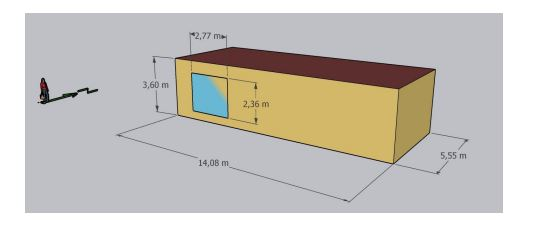
\includegraphics[scale=1.5]{building.JPG}
    \centering
    \caption{3D model of the case study building}
    \label{fig:building}
\end{figure}

\noindent
The building is 14.08 meters long, 5.55 meters wide and 3.60 meters high as shown in figure\ref{fig:building}.The window has a height of 2.36m and a width of 2.77m. The dimensions of the building are summarized in Table\ref{table:building}

\begin{table}[H]
\centering
\begin{tabular}{|c|c|c|}
\hline \text { Building dimension } & \text { Value }\\
\hline \text { Length } & 14.08 m\\
\hline \text { Width } & 5.55 m\\
\hline \text { Height } & 3.60 m\\
\hline \text { Volume } & 281.32 m^{3}\\
\hline \text { Floor area } & 78.14 m^{2}\\
\hline
\end{tabular}
\caption{Dimensions of case study building}
\label{table:building}
\end{table}

\noindent
Concerning the materials, walls, windows, floors and ceilings are made of several layers of different materials and thickness, that will be listed from the outside layer to the inside layer. Walls are made of a 9cm thick concrete layer,followed by a 6cm thick mineral wool layer, a 14cm concrete layer and a 12cm Multipor (insulation material) layer. The ceiling is made of a 2.5cm Fermacell (gypsum) layer, followed by a 4cm Polyurethane layer and a 20cm concrete layer.
The floor is made of a 18cm concrete layer, followed by a 4cm insulation layer, a 6cm concrete layer and a 4mm floor covering layer. The window is made of a 6mm clear float glass sheet,followed by a 15mm of Argon layer and again a 6mm clear float glass sheet.

\subsection{Time Step }
Specifies the  time step for the simulation calculations.The value entered here is the number of time steps to use within an hour. Longer length time steps have lower values for Number of time steps per Hour. For example a value of 6 entered here directs the program to use a zone time step of 10 minutes.The choice of the time step has important implications for modeling accuracy and the overall time it takes to run a simulation.The time step should be evenly divisible into 60.The choice made was a time step of 10 minutes for the simulations because it was the shortest time step that guaranteed accurate results.The time step is by default the sampling period $T_{s}$ of the input and output.

\subsection{Electric Equipment}
The building is equipped with an electric heater whose behaviour is modelled by the Electric Equipment object in EnergyPlus.The difference between an Electric Equipment and HVAC system is that it is possible to choose manually the value of the power delivered by the Electric Equipment
whereas with the HVAC, it is not possible for the user to act on its delivered power but only on the temperature set points of the thermostat.In addition, the thermostat already implements an internal control scheme (on/off) while the final goal is to implement a more advanced controller.The properties of the electric heater are given in Table\ref{table:Heater}.A radiant fraction of 0.5 corresponds to a single column heater. It is assumed that there isn’t any heat, produced by the heater, that is lost towards the outside of the building.The convective fraction is expressed as $F_{\text {convective }}=1-\left(F_{\text {latent }}+F_{\text {radiant }}+F_{\text {lost }}\right)$ and equals 0.5 where $F$ stands for fraction.

\begin{table}[H]
\centering
\begin{tabular}{|c|c|c|}
\hline \text { Property } & \text { Value }\\
\hline \text { Max Power } & 14.08 m\\
\hline \text { Latent fraction  } & 5.55 m\\
\hline \text { Radiant fraction  } & 3.60 m\\
\hline \text { Lost fraction } & 281.32 m^{3}\\
\hline \text { Convective fraction  } & 78.14 m^{2}\\
\hline
\end{tabular}
\caption{Properties of the Heater}
\label{table:Heater}
\end{table}

\subsection{Infiltration and Ventilation}
Infiltration and ventilation are two different types of sources of flow of air in a
building.Infiltration is the unintentional or accidental introduction of outside air into a building, typically through cracks in the building envelope and through use of doors for passage.It is sometimes called air leakage. In contrast,ventilation is a flow of air that is intentional.Ventilation can be either natural, by opening a window for example, or forced due to an HVAC system.Infiltration and ventilation have been taken into account in the building. However, no forced ventilation is considered, only natural ventilation, since the building is not equipped with fans or HVAC system.Typical values of a building the size of our case study building are  an infiltration rate of 0.0156 $m^{3}/s$ and a natural ventilation rate of 0.0391 $m^{3}/s$


\newpage
\section{System Identification}
In this section some notions of system theory and identification used in this thesis are recalled.Firstly the definition of  what are Linear Time-Invariant (LTI) systems and their models.Then Models with non-linearity will be discussed afterwards we will discuss Transfer function estimation , model validation and stability. 

\subsection{LTI Systems}

The notion of a system is a broad concept.A system operates on an input signal to produce an output signal.The output is an observable signal that is of interest to us.Within the inputs we can distinguish the ones that can be manipulated by the observer from disturbances.The disturbances can be divided into those that are directly measured and those that are only observed through their influence on the output.The distinction between inputs and disturbances is often of less importance in the modelling process.

Systems can be classified on the dependence of the current outputs with respect to previous ones.Dynamic systems are systems which current output not only depends on the current input but also on past outputs.They are said to have memory.In this thesis we are dealing with a dynamic system.Figure \ref{fig:system representation} shows the representation of the system with inputs $u$, output $y$ and system model $G$

\begin{figure}[H]
    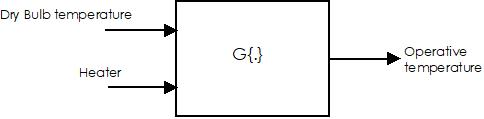
\includegraphics[scale=1]{system.jpeg}
    \centering
    \caption{Representation of the system}
    \label{fig:system representation}
\end{figure}


Linear Time-Invariant systems are systems that are Time-invariant and where the superposition principle holds.superposition principle means that the response of an LTI system behaves as follows:
    
\[y_{1}(t)=G\left\{u_{1}(t)\right\} \]
\[y_{2}(t)=G\left\{u_{2}(t)\right\} \]
\[a y_{1}(t)+b y_{2}(t)=G\left\{a u_{1}(t)+b u_{2}(t)\right\}\]

Time-Invariance property means that the response does not depend on the time at which the excitation has been applied.A time-delay on the input produces an equivalent
time-delay on the output.

\[y(t)=G\left\{u_(t)\right\} \]
\[y(t-\tau)=G\{u(t-\tau)\}\]

Causality property is also of interest.A causal system means that the response of the system cannot depend on an excitation in the future.We supposed that our system was a causal LTI system. 

\subsection{Response of LTI Systems}
Any  continuous-time dynamic system can be described by a differential equation and a discrete-time dynamic system by a difference equation as follows:



\[\sum_{k=0}^{n_{a}} a_{k} \frac{d^{k} y(t)}{d t^{k}}=\sum_{k=0}^{n_{b}} b_{k} \frac{d^{k} u(t)}{d t^{k}} \]

In continuous-time ($t$ $\in \mathbb{R}$)

\[\sum_{k=0}^{n_{a}} a_{k} y(n-k)=\sum_{k=0}^{n_{b}} b_{k} u(n-k)\]

In discrete-time  ($n$ $\in \mathbb{Z}$)


Using the Laplace transform for the continuous-time case and the Z transform for the discrete case one can obtain the transfer function $G$ which characterizes completely the system.The response of the system is expressed as follows:

\begin{equation}\label{eq:sys.response}
Y(j\omega)=G\left(j\omega\right) U(j \omega)+T^{\circ}(j\omega)
\end{equation}

where $G\left(j\omega\right)$ is system's transfer function, $U(j \omega)$ and $Y(j\omega)$ the input and output DFT spectra, $T^{\circ}(j\omega)$ the transient term and $j \omega$ a frequency complex variable.

The first term of \eqref{eq:sys.response} is the steady-state response of the system.In the time domain, the transient term is exponentially decaying.It is actually the free response of the system that is the response when the input is zero in the measured time window.Therefore, when $t\rightarrow \infty$ that is at steady-state the system response is fully described by the transfer function response.

It can be interesting to look into the particular class of periodic excitation. A Sinusoidal function is a sum of complex exponential:

\[\sin (\omega t+\phi)=\frac{e^{j(\omega t+\phi)}+e^{-j(\omega t+\phi)}}{2 j}\]

The response of an LTI system to a complex exponential  is a scaled version of the same complex
exponential:

\[G\left\{e^{j \omega t}\right\}=e^{j \omega t} G(j \omega)\]

We therefore have that the response of an LTI system to a sine wave is also a sine wave  with same
frequency as input, but with a different amplitude and phase.The complex exponential signal is therefore an eigenfunction of the system and $G(j \omega)$ evaluated at the frequency of the input is the corresponding eigenvalue of the system.$G(j \omega)$ being a complex-valued function, it can be split into an amplitude function A and a phase function $\Phi$:

\[G(j \omega)=A(\omega) e^{j \Phi(\omega)}\]

If we apply an input signal of the form $u(t)=\sin (\omega t+\phi)$, then the output is given as:


\[y(t)=G\{\sin (\omega t+\phi)\} =A \sin (\omega t+\phi+\Delta \phi)\]
\[A =|G(\omega)| \]
\[\Delta \phi =\angle G(\omega)\]

Where A and $\Delta \phi$ are  the amplitude  and phase of the transfer function respectively.By applying a sine to an LTI System we can easily characterize the system.Fig\ref{fig:single sine} shows the result in the time domain of a heater sine wave of RMS value 1.4kW applied to our system.

\begin{figure}[H]
    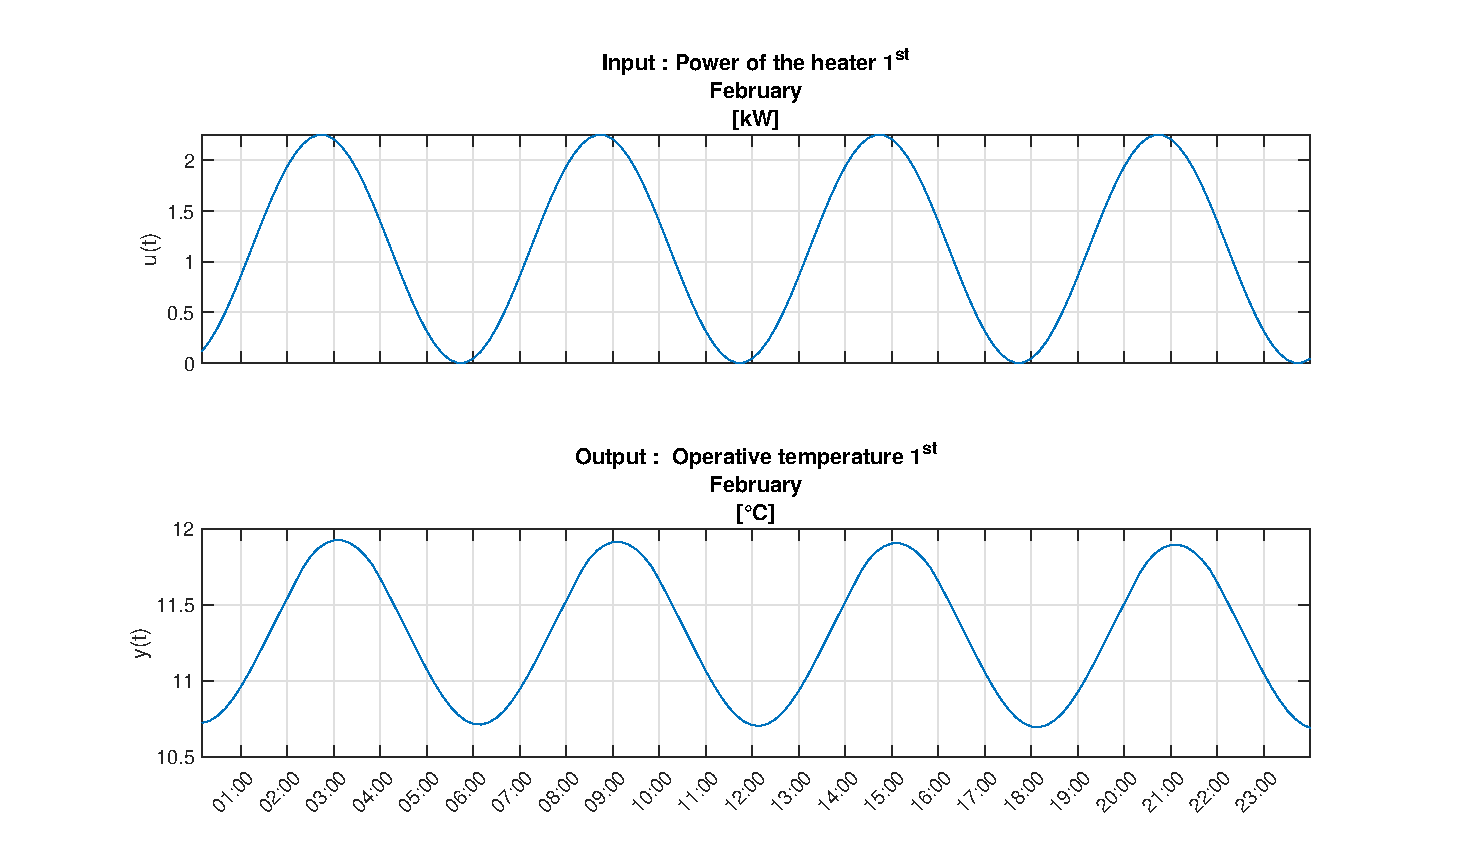
\includegraphics[scale=0.7]{single_sine_rms_1400.eps}
    \caption{Response of the system to a sinusoidal heater input of RMS value 1.4kw}
    \label{fig:single sine}
\end{figure}

We can see from the result that the output to the sine excitation is also a sine wave with no phase shift.For this signal excitation level,the LTI assumption hold true.

\subsection{Nonlinear models}
Since most of the relationships in physics are nonlinear,nearly all systems are inherently nonlinear in nature.In reality the linearity assumption is only approximately valid.Most systems are only linear to a first approximation.Moreover,they are a special case of nonlinear systems in limited ranges of operation.Fig\ref{fig:examplenonlinear} shows some examples of nonlinear relationships.


\begin{figure}[H]
    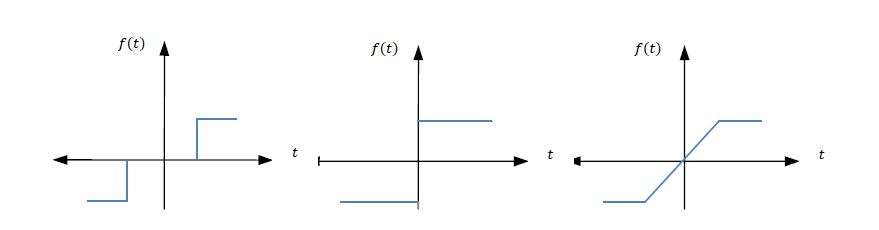
\includegraphics[scale=1]{examplenonlinear.JPG}
    \centering
    \caption{some examples of nonlinear relationships}
    \label{fig:examplenonlinear}
\end{figure}



Depending on the excitation level, the output is disturbed by nonlinear distortions so that the linearity assumption no longer holds.The term nonlinear distortions indicates that nonlinear systems with a linear term are considered. The deviations from the linear behavior are called nonlinear distortions.The goal of this section is not to show how nonlinear systems should be modeled but provide an insight on how nonlinear distortions can impact the validity of the obtained models.

Let us consider an excitation signal

\[u(t)=\sum_{m=1}^{K} A_{m} \cos \left(\frac{2 \pi m}{T} t+\phi_{m}\right)\]
\[\omega=\frac{2 \pi m}{T}\]

This signal is called a multisine because it consists of a sum of sines.Since it is a periodic excitation, the considerations on the response of such signals stated above also apply.To detect the nonlinear behaviour a periodic excitation is needed.Considering a nonlinear system $y=u^{\alpha}$ excited by a multisine at the frequencies $\pm \omega_{k}, k=1, \ldots, F$ and remembering that a signal has  positive and negative frequencies and that multisines are sum of complex exponentials the output will yield products of exponentials.The frequencies at the output of such a system are given by making all possible combinations of $\alpha$ frequencies, including repeated frequencies, selected from the set of 2F excited frequencies.

\[\sum_{i=1}^{\alpha} \omega_{k_{i}}, \text { with } \omega_{k_{i}} \in\left\{-\omega_{F}, \ldots,-\omega_{1}, \omega_{1}, \ldots, \omega_{F}\right\} \text {. }\]

Further,the components at $n\omega_{k_{i}}$ with $n > 1$ are the harmonics of $\omega_{k_{i}}$ and the ones obtained by combinations of the harmonics are the intermodulation products.The harmonics and intermodulation products are often unwanted. Therefore, we refer to these signals as nonlinear distortion.

To detect the nonlinearities the idea is to design a multisine  that excites a well-selected set of odd frequencies.Odd frequencies correspond  to odd values of $i$ in the summation above.Even nonlinearities show up at the even frequencies because an even number of odd frequencies is added together. Odd nonlinearities are present only at the odd frequencies because an odd number of odd frequencies is added together. At the odd frequencies that are not excited at the input, the odd nonlinear distortions become visible at the output because the linear part of the model does not contribute to the output at these frequencies.By using a different color for each of these
contributions, it becomes easy to recognize these in an amplitude spectrum plot of the output signal. Fig \ref{fig:MS_1.4},  Fig \ref{fig:MS_2.5} and  Fig \ref{fig:MS_4.0} shows the result of three simulations obtained with different multisine heater  excitation levels.

\begin{figure}[H]
    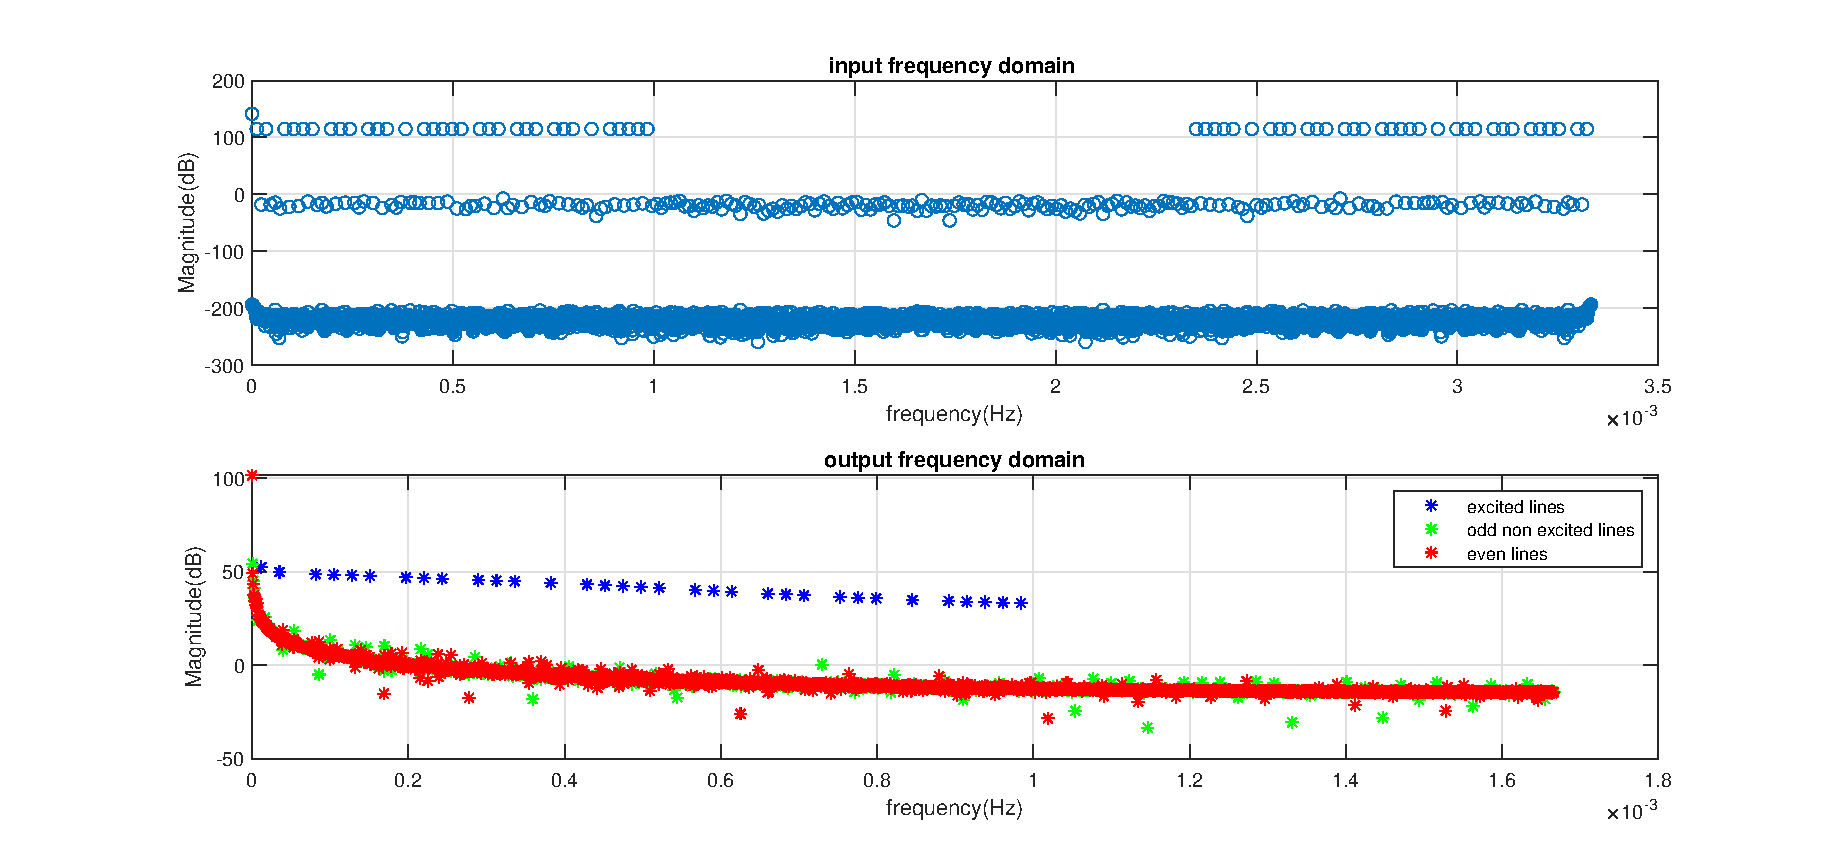
\includegraphics[scale=0.6]{fdomain_input_rms_1400.eps}
    \centering
    \caption{Multisine with RMS value of 1.4 kW}
    \label{fig:MS_1.4}
\end{figure}

\begin{figure}[H]
    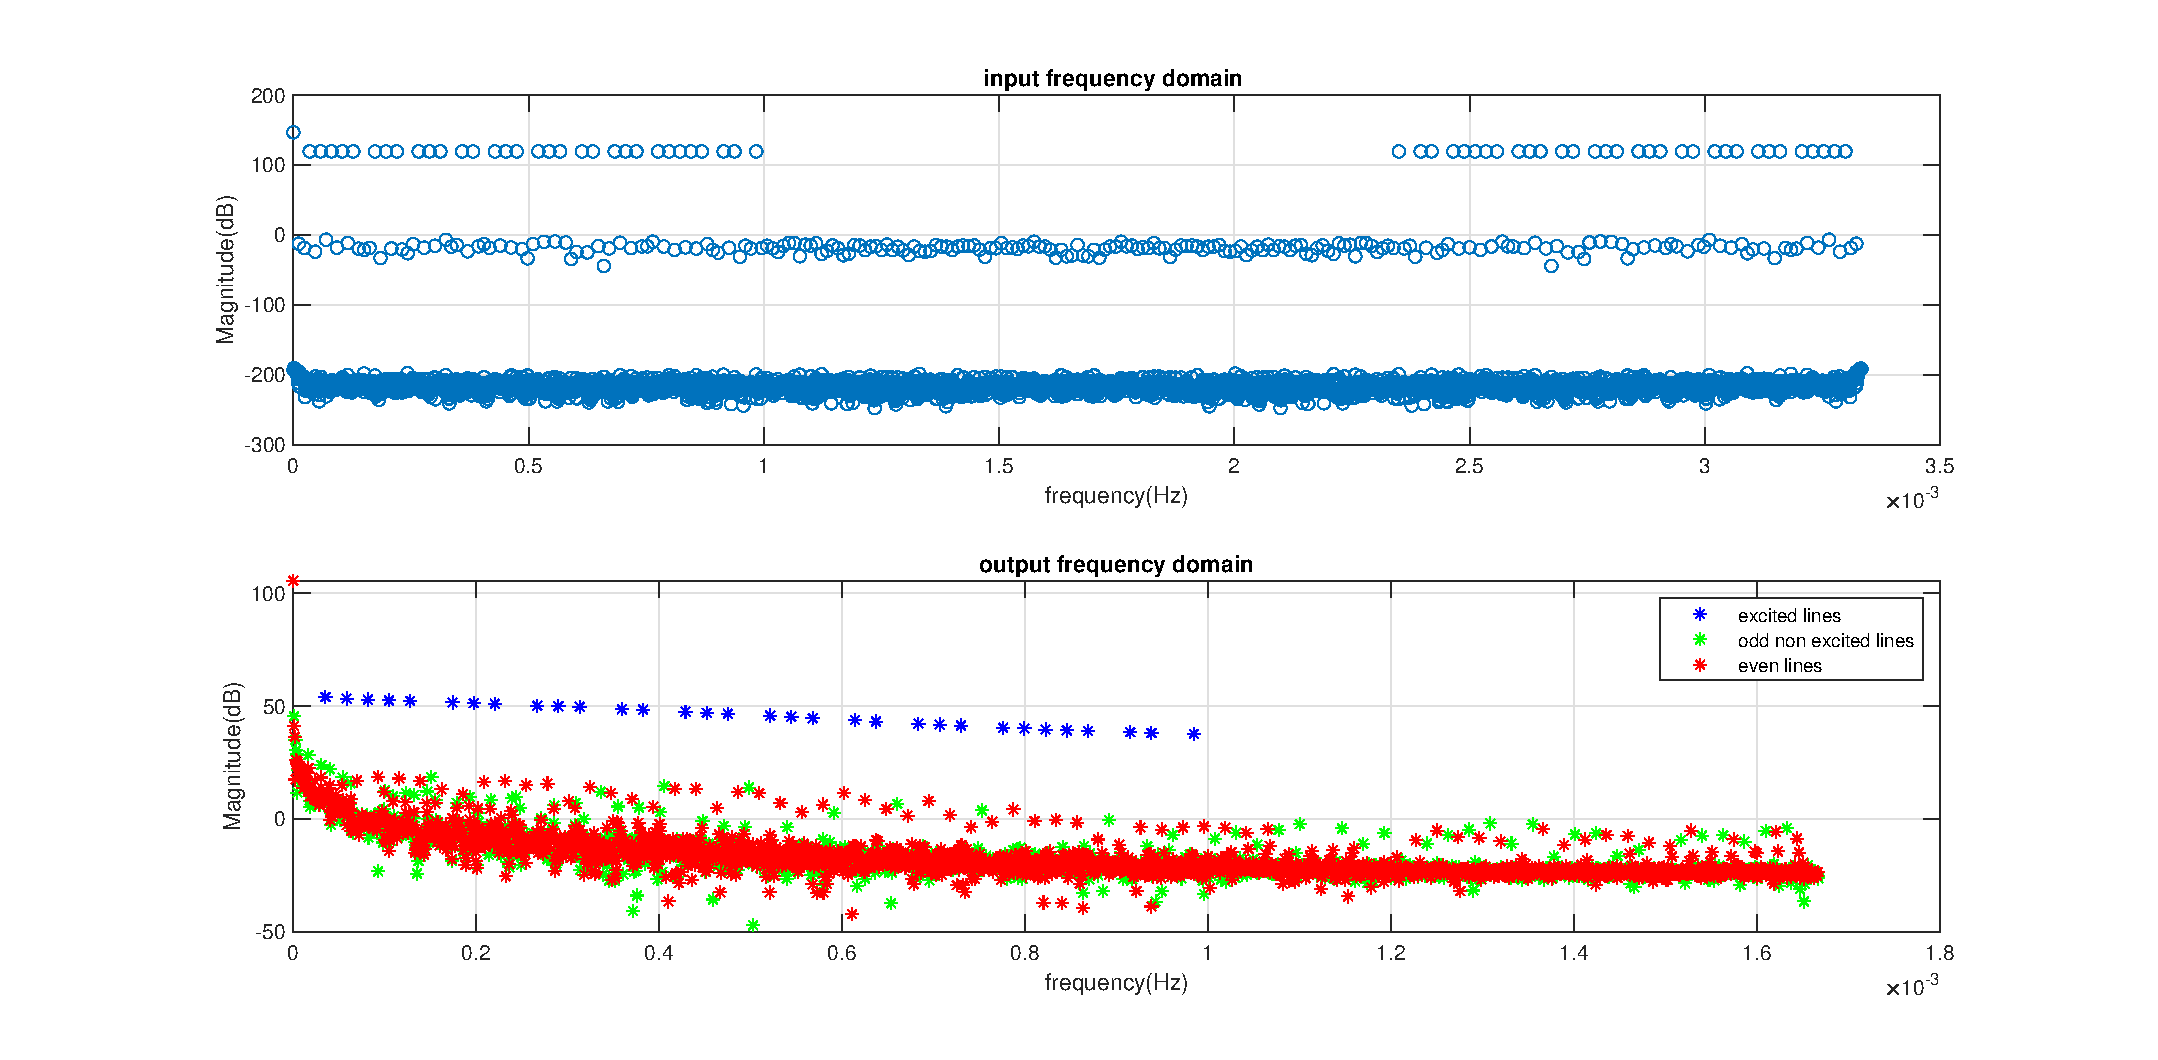
\includegraphics[scale=0.5]{fdomain_input_rms_2500.eps}
    \centering
    \caption{Multisine with RMS value of 2.5 kW}
    \label{fig:MS_2.5}
\end{figure}

\begin{figure}[H]
    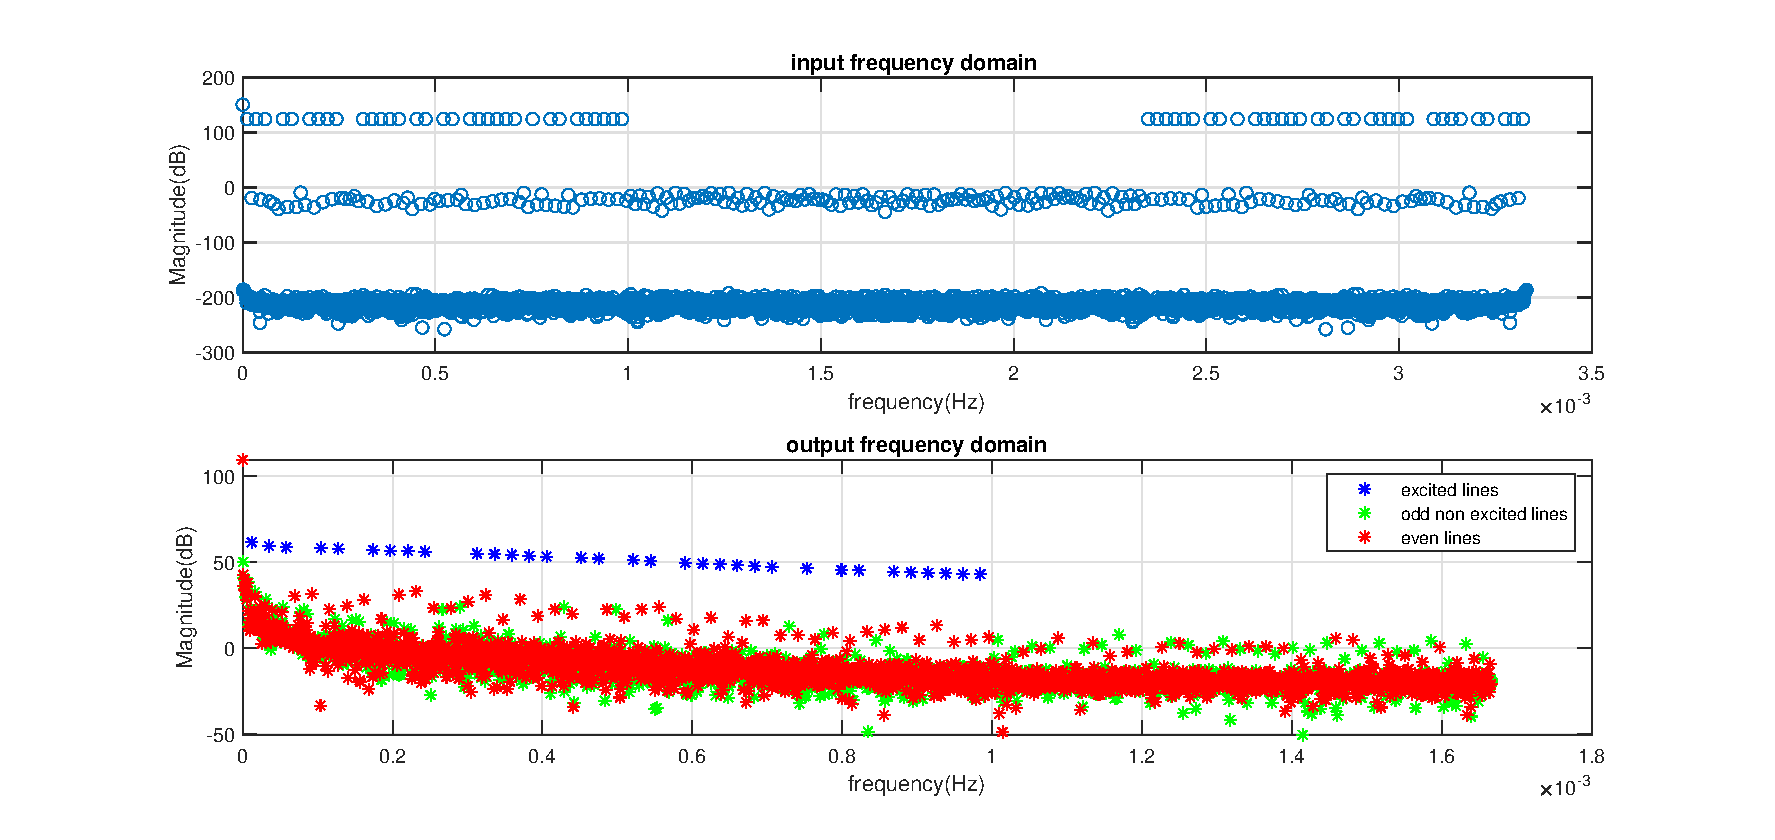
\includegraphics[scale=0.6]{fdomain_input_rms_4000.eps}
    \centering
    \caption{Multisine with RMS value of 4 kW}
    \label{fig:MS_4.0}
\end{figure}

From the reults we can notice that as the excitation level increases the nonlinearities also increases.The system is subject to nonlinearities.The blue contribution is the response of the system to the excited input frequencies ie the Linear response contribution.The green dots correspond to the odd non excited nonlinear contributions.We also notice the appearance of a smooth red contribution at the output.This contribution is due to the transient and even nonlinearities.As long as the the ratio of the level of the nonlinearities to the level of thelinear contribution is proper one can assume the LTI assumption to hold true.




\subsection{System Identification procedure}
Identification session consists of a series of basic steps.In each session the following actions should be taken:
\begin{itemize}
    \item Collect information about the system.
    \item Select a model structure to represent the system.
    \item Choose the model parameters to fit as well as possible the model to the measurements:
selection of a goodness of fit criterion.
     \item Validate the selected model.
\end{itemize}

\subsubsection{Information collection}
Building a model requires one should first get information about the system.This can be done by just observing the natural dynamics of the system for example vibration analysis of a bridge that is excited by normal traffic,but most often it is more efficient to set up dedicated experiments that actively excite the system for example like the controlled excitation of a mechanical structure using a shaker.The controlled excitation has to be selected to optimize  goals  for example like minimum time, minimum time, or minimum power consumption of the experiment within operator constraints like the excitation should remain below a maximum allowable level as we saw in previous sections.

Additionally, data pre-processing and pre-filtering  may be necessary as the collected data in its raw form is not usually ready to be used for model development.Aside from noise that affects data quality two other factors like outliers and missing data may have to be dealt with.Outliers is data that do not conform to other parts of the data largely due to sensor malfunction while  missing data which may be due to power disruption,sensor malfunctioning or data transfer losses. 

Handling outliers might be tricky and rely on statistical methods.Nevertheless, if the input excitation signal is periodical and if multiple period measurement are available then we can simply replace the value we suspect to be an outlier with the value from another period.Missing data can be handled by interpolating the value between the two nearest neighbours of the missing one.As for pre-filtering it may be desirable to emphasize fits over a specific frequency range either due to the needs of that application and/or it is known that the noise dominates the measurement outside this band.In either case  filtering the measurements prior to identification may be useful.

\subsubsection{Model Structure Selection}
Multiple mathematical models can be used to represent a system.A choice should be made within the wide variety of possibilities such as:

\subsubsection*{ Non-parametric models versus Parametric models }
The term non-parametric does not imply that the model does not have unknowns or parameters.It implies that the model do not have any mathematical structure for the response of the system.As an example let us consider the step response model of a system, which is simply the set of step response coefficients at the sampling instants.In a Non-parametric model the system is characterized by measurements of a system function at a large number of points If the system is assumed to have first-order characteristics, then the response can be characterized by three parameters, namely, gain,time-constant and time-delay.When the response coefficients are directly estimated, it is termed as non-parametric identification.FRF(Frequency response function) measurement is another example of non-parametric model.Fig shows the impulse response of a system at a large number of points.

\begin{figure}[H]
    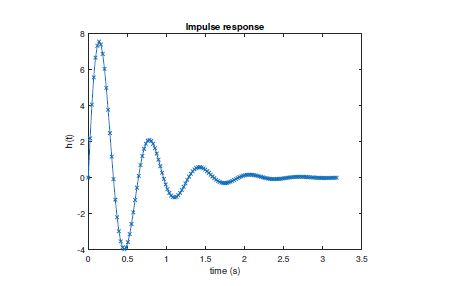
\includegraphics[scale=1]{impulse_response.JPG}
    \centering
    \caption{impulse response of a system at a large number of points}
    \label{fig:imp_res}
\end{figure}


The term parametric refers to the parametrization of the model.The system is described using a limited number of characteristic quantities called the parameters of the model.They possess a  specific structure and order.An example of a parametric model is a transfer function,where the parameters are the coefficients of the polynomials defining the numerator and the denominator.primarily three broad classes of parametric model families exist,
namely, the equation-error , output-error and the Box-Jenkins family.

The Equation-eerror models is made-up of a system model $G$ and noise model $H$ and has different structures (ARX,ARMAX,ARMA).The output-error assumes that the noise directly affects the output.The Box-Jenkins resorts to an independent parametrization of the system and noise models.Fig\ref{fig:par_res} shows the representation of a parametric input-output relationship.

\begin{figure}[H]
    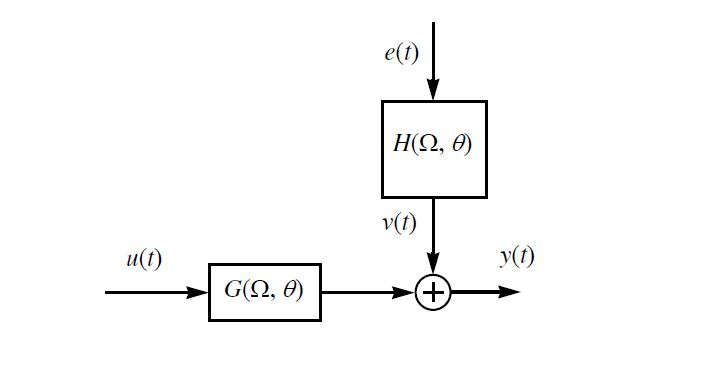
\includegraphics[scale=1]{parametric_repre.JPG}
    \centering
    \caption{representation of a parametric input-output relationship}
    \label{fig:par_res}
\end{figure}

\begin{equation}\label{eq:trfctmodels}
Y(k)=G\left(\Omega_{k}, \theta\right) U(k)+T_{G}\left(\Omega_{k}, \theta\right)+H\left(\Omega_{k}, \theta\right) E(k)+T_{H}\left(\Omega_{k}, \theta\right)    
\end{equation}


\noindent
where
\[G(\Omega, \theta)=\frac{B(\Omega, \theta)}{A(\Omega, \theta)}, T_{G}(\Omega, \theta)=\frac{I_{G}(\Omega, \theta)}{A(\Omega, \theta)}, H\left(\Omega_{k}, \theta\right)=\frac{C(\Omega, \theta)}{D(\Omega, \theta)}, T_{H}(\Omega, \theta)=\frac{I_{H}(\Omega, \theta)}{D(\Omega, \theta)}\]

\noindent
and the numerators and denominators of the expressions polynomials
\[\Omega_{k}=j\omega_{k}\]
\[\theta:\;parameters\]
\[ARX:\; C=1,\; D=A,\; T_{H}=0\]
\[ARMAX:\; D=A,\; T_{H}=0 \]
\[ARMA:\; G=0,\; T_{G}=0\]
\[OE:\; G(\Omega, \theta)=\frac{B(\Omega, \theta)}{F(\Omega, \theta)},\;\;H=1 ,\;\; T_{H}=0  \]
\[BJ:\; D \neq A\]


Non-parametric models can be estimated with minimal a priori knowledge while the estimation of parametric models demands some a priori knowledge.The a priori knowledge needed can be obtained from physical insight of the system.It can also be acquired by first estimating a non-parametric model.

\subsubsection*{ White box models versus black box models }
White box models are models that require specialized knowledge related to a scientific field.That is the modelling requires understanding of physical laws such as for example Kirchhoff’s and Newton’s laws.The white box model is often used to gain insight into working principles of a system and they are those models that are used in simulation softwares.

Black box models do not require detailed study using physical laws of the system to obtain a model.The model is estimated  using only the observed input and output measurements.Black box models are usually used when only output prediction of the system is needed. 

\subsubsection*{ Linear models versus nonlinear models }
Linear system identification framework has seen much more development and is more complete than the nonlinear identification framework that  requires more data and is more involved.In real life almost every system is nonlinear and  can be linearised around an operation region to obtain a linear model which is more simpler to handle.The choice of model depends on if the linear behaviour is dominant or not.

\subsubsection*{ Linear-in-the-parameters versus nonlinear-in-the-parameters }
A model is called linear-in-the-parameters if there exists a linear relation between these parameters $\theta$ and the error $\epsilon$ that is minimized.

\[\epsilon=y-K(u) \theta\]
\[K \in \mathrm{R}^{N \times n_{\theta}}\]

Linearity in the parameters has a strong impact on the complexity of the estimators such that the optimization problem that can be solved analytically  otherwise an iterative optimization has to be performed.

\subsubsection{ Estimation}
Once a model structure is chosen,the estimation can then be carried out.Using the observed information about the system and the model structure, an optimization problem has to be solved that minimizes a criterion characterizes the point of optimum in the search.

Several estimation method exists and the choice of the optimization criterion determines the stochastic properties of the estimator such as the bias, variance and consistency.An example of estimation method is the Least squares method which has the generic form

\[\min _{\theta}\left\|\mathbf{y}_{N}-\hat{y}(\theta)\right\|_{2}^{2}\]

\noindent
where $\mathbf{y}_{N}$ is the vector of stacked measurements, $\hat{y}(\theta)$ is the predictor expression resulting from a model and $\theta$ are the vector of model parameters.

\subsubsection{Model validation}
The validity of the model obtain should be accessed.We need to know if the model describes well the dynamics of the system.Usually the available data for the modelling exercise is partitioned in 2 data sets.An estimation set and a validation set.Modelling errors are errors due to the model's inability  to predict the  validation data set .There might be several reasons to this.One reason can be over-fitting of the estimation data set thereby equally modelling noise.The choice of the model structure might not be the right one.The estimation data set might not be informative enough and therefore a new data set is required.Non-linear distortions might also be a reason, a new model structure should then be chosen.The Identification framework being iterative,the procedure might be done several times before obtaining a proper model. 

\newpage
\section{Method}
This section deals with details of the various methods as well as the results obtained using the methods to obtain models.As showed in the previous chapters the dynamics from heater to operative temperature and the one from Dry bulb temperature to operative temperature are not the same.By estimating  a transfer matrix instead of a transfer function one could obtain a better system model.The expression of the input-output relationship will then be as follows:

\begin{gather}
Y(k)=G_{1}\left(\Omega_{k}, \theta\right) U_{1}(k)+G_{2}\left(\Omega_{k}\theta\right) U_{2}(k)+T_{G}\left(\Omega_{k}, \theta\right) \label{eq:matrix form}\\
Y=\mathbf{G}U + T
\end{gather}

\noindent
Where $ U_{1}(k)$ and $ U_{2}(k)$ are the DFT of the heater input and Dry bulb temperature respectively. $Y(k)$ the DFT of the output.$G_{1}$ and $G_{2}$ are the transfer function from heater to operative temperature and the transfer function from dry bulb temperature to operative temperature respectively.$\mathbf{G}=$
 $\begin{bmatrix}
  G_{1} & G_{2}\\ 
\end{bmatrix}$, $U=$
 $\begin{bmatrix}
  U_{1}\\ 
  U_{2}
\end{bmatrix}$, $Y$, $U_{1}$ and $U_{2}$ $\in \mathrm{R}^{1 \times N}$. N the number of data samples.

Using the Building defined in EnergyPlus, the system is simulated.We have two inputs, one controllalable that we can design and another one uncontrollable.These two inputs are taken into account by EnergyPlus and the operative temperature is computed by the software.Then using the output from EnergyPlus we can carryout the Identification procedures using Matlab to obtain our models.Fig shows a schematic of the procedure.


From \ref{eq:matrix form} we can see that there is at least two models to estimate $G_{1}$ and $G_{2}$ and as we assumed the system to be an LTI one superposition principle holds true and then we might do the two models identification separately.For each model estimation, we will discuss the excitation design if it is a controllable input, the model structure, the estimation method, results and model validation.

\subsection{Data preprocessing}
When the data is collected from the simulation software it is not in shape for immediate use in the identification algorithms.Some operations needs to be done on the data.All the estimated method used in the identification are frequency domain methods.

The first operation is then obviously to transform the data from the time domain to the frequency domain.To do so we apply the  Discrete Fourier Transform (DFT) on the time domain input and output signals:

\begin{equation}
\begin{array}{rll}
u(t) & \stackrel{\mathrm{DFT}}{\longrightarrow} & U(j \omega) \\
y(t) & \stackrel{\mathrm{DFT}}{\longrightarrow} & Y(j \omega)
\end{array}
\end{equation}

\noindent
where the time and frequency vectors are given by :

\begin{equation}
\begin{aligned}
t &=T_{s}\left[\begin{array}{lllll}
0 & 1 & 2 & \cdots & N
\end{array}\right] \quad \mathrm{s} \\
\omega &=\frac{2 \pi}{N T_{s}}\left[\begin{array}{lllll}
0 & 1 & 2 & \cdots & N
\end{array}\right] \quad \mathrm{rad} / \mathrm{s}
\end{aligned}
\end{equation}

The DFT conjugate symmetry property says that there is redundancy in the spectral content of a real-valued signal.The DFT of a  real-valued signal with $N$ samples has also $N$ samples.The conjugate symmetry implies that  the signal can be fully represented by a minimal set of frequencies $M$ smaller than $N$. $M$ depends on whether N is even or odd. The gain in using this property is when $N$ is large as there is a cut down in memory consumption and processing time. $M$ is obtained using the formula 

\begin{equation}
M=1+\left\lfloor\frac{N}{2}\right\rfloor   
\end{equation}


\noindent
where $\lfloor\cdot\rfloor$ is the floor operator: the largest integer no greater than its input.The frequency vector becomes :

\begin{equation}
\begin{aligned}
\omega &=\frac{2 \pi}{N T_{s}}\left[\begin{array}{lllll}
0 & 1 & 2 & \cdots & M
\end{array}\right] \quad \mathrm{rad} / \mathrm{s}
\end{aligned}
\end{equation}

The thermal behaviour of a building being a slow process implies that the main information on the dynamics of the system is the low frequency components and that we should emphasize the modelling on the low frequency components.We therefore can only take into account the first few frequencies of the input-output spectra.The optimal new $M$ is to be obtained by iteration.

\subsection{System Linearization}
As we mentioned earlier systems in practice are nonlinear and are only linear in a limited range of operation.A linearization around a nominal operating point is then necessary.The objective of the linearization  is to derive a linear approximate system whose response will agree closely with that of the original nonlinear system which it comes from. By considering small variations around our nominal operating point($u_{o}$,$y_{o}$)

\begin{equation}
\begin{aligned}
&y(t)=y^{m}(t)-y_{o} \\
&u(t)=u^{m}(t)-u_{o}
\end{aligned}
\end{equation}

\noindent
Where $y^{m}$ and $u^{m}$ are the output and input time domain samples obtained from EnergyPlus. $y_{o}$,$u_{o}$ the mean value of $y^{m}$ and $u^{m}$ respectively. Then substituting this deviations into our nonlinear relationship $y=f(u)$. Fig\ref{eq:linearization} shows the linearization of $y=f(u)$ at an operating point ($u_{o}$,$f(u_{o})$)

\begin{figure}[H]
    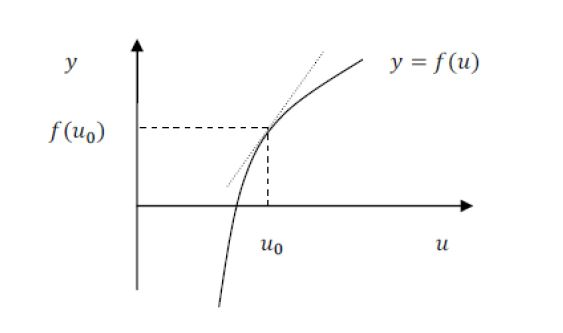
\includegraphics[scale=1]{linearization.JPG}
    \centering
    \caption{linearization of $y=f(u)$ at an operating point ($u_{o}$,$f(u_{o})$)}
    \label{eq:linearization}
\end{figure}

After linearization the frequency vector becomes:

\begin{equation}
\begin{aligned}
\omega &=\frac{2 \pi}{N T_{s}}\left[\begin{array}{lllll}
1 & 2 & \cdots & M
\end{array}\right] \quad \mathrm{rad} / \mathrm{s}
\end{aligned}
\end{equation}

\subsection{Identification of Heater Model G1}
To obtain $G_{1}$ we will first obtain a non-parametric model of the system from Heater to operative temperature.This non-parametric model Will then be used to obtain the parametric one $G_{1}$.

\subsubsection{ Excitation design }
When we have a choice in the input signal to be used in the identification, optimization of the excitation signal both in the time domain and frequency domain can be made.Optimizing in the time domain results in a minimum crest factor.The crest factor is defined as

$$
\text { crest factor }=\frac{\text { peak value }}{\text { effective RMS value }}
$$

The effective RMS value $V_{RMSe}$ is given by

$$
V_{R M S e}=V_{R M S} \sqrt{\frac{\text { energy at the frequencies of interest }}{\text { total energy of the excitation }}}
$$

\noindent
This results in an improved signal-to-noise(S/N) ratio, hence greater accuracy in the estimates.An optimal power spectrum can be obtained from the frequency domain.This results in an optimal distribution of the of the available energy of the excitation signal resulting in a minimal uncertainty on the estimates.

The multisine was chosen as excitation signal.It allows generation of an optimum power spectrum with a minimum crest factor.Additionally the multisine can also be used to detect nonlinear distorsions as discussed earlier.The spectral resolution $f_{o}$ of the multisine should be chosen high enough so that no sharp resonances are missed.Since $f_{0}=1 / T_{s}$ , it sets immediately the period length $T_{s}$ of the multisine. A high-frequency resolution requires a long measurement time because at least one, and preferably a few, periods should be measured.Unfortunately we are limited in the frequency resolution as the $T_{s}$ is limited in EnergyPlus.

\subsubsection{ Model structure }
The choice of the model depends on the aim of the model.The aim of the model is for control purposes.With regard to this the choice made was a continuous time parametric black-box model.

\subsubsection{Estimation Method Non-parametric model}
The Non-parametric model to be determined is a Frequency Response Function (FRF).Using a multisine,  characterization of the nonlinear distortions is also possible and we will describe the Robust method which enables its characterization in the next paragraph.In pratice data is obtained from measurements and noise is present.To obtain the FRF, averaging techniques are often used to reduce FRF measurements errors.Starting from $M$ successive periods of  input-output data blocks $u^{[l]}(t), y^{[l]}(t), \quad l=1,2, \ldots, M$ the inputs and outputs are averaged over those periods to obtain sample mean and sample covariances and the FRF estimate is given as

\begin{equation}
\hat{G}\left(j \omega_{k}\right)=\frac{\hat{Y}(k)}{\hat{U}(k)}
\end{equation}

\noindent
Where the sample mean and sample covariances are given as

$$
\hat{U}(k)=\frac{1}{M} \sum_{l=1}^{M} U^{[l]}(k), \quad \hat{Y}(k)=\frac{1}{M} \sum_{l=1}^{M} Y[l](k)
$$

$$
U^{[l]}(k)=\operatorname{DFT}\left(u^{[l]}(n)\right), \quad Y^{[l]}(k)=\operatorname{DFT}\left(y^{[l]}(n)\right)
$$

\begin{equation}\label{eq:covar}
\begin{aligned}
&\hat{\sigma}_{U}^{2}(k)=\frac{1}{M-1} \sum_{l=1}^{M}\left|U^{[l]}(k)-\hat{U}(k)\right|^{2}, \hat{\sigma}_{Y}^{2}(k)=\frac{1}{M-1} \sum_{l=1}^{M}\left|Y^{[l]}(k)-\hat{Y}(k)\right|^{2} \\
&\hat{\sigma}_{Y U}^{2}(k)=\frac{1}{M-1} \sum_{l=1}^{M}\left(Y^{[l]}(k)-\hat{Y}(k)\right)\left(\overline{U^{[l]}(k)-\hat{U}(k)}\right)
\end{aligned}
\end{equation}

The aim of the robust method is to obtain the best linear approximation $G_{BLA}$, the linear system that fits best the data and the nonlinear noise, the contribution of nonlinear distortions and noise.Starting from multiple experiments with odd random phase multisines, for each experiment a number of consecutive a number of consecutive periods of the steady state response are measured, and the FRF corresponding to each period is calculated.Averaging of the FRFs over the consecutive periods quantifies the noise level.Averaging of these mean FRFs over the multiple experiments quantifies the sum of the remaining noise level and the level of the stochastic nonlinear distortions. Finally, the difference between the total distortion level (averaging over the experiments) and the noise level (averaging over the periods) is an estimate of the stochastic nonlinear distortions.The whole
procedure is summarized in Figure\ref{fig:robust procedure}

\begin{figure}[H]
    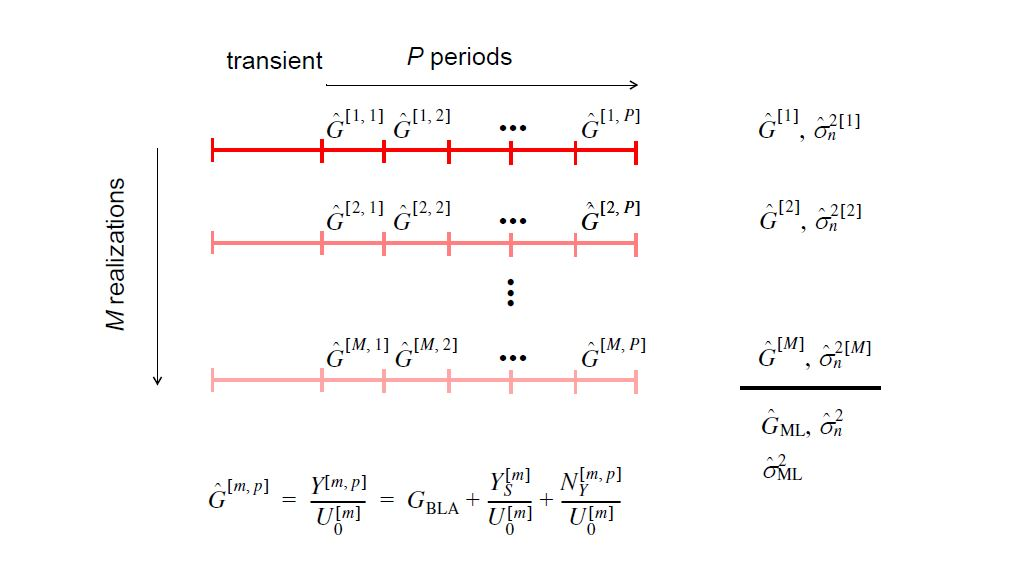
\includegraphics[scale=0.9]{robust_procedure.JPG}
    \centering
    \caption{The robust procedure for estimating $G_{BLA}$}
    \label{fig:robust procedure}
\end{figure}

\noindent

$\hat{G}[m, p]$ is the FRF estimate of the $p$th period of the $m$th experiment, which depends on the BLA $G_{BLA}$, the stochastic nonlinear distortions $G_{S}^{[m]}$, and the noise $N_{G}^{[m, p]}$.$ \quad \hat{G}^{[m]}, \hat{\sigma}_{n}^{2[m]}$ are, respectively, the sample mean and sample noise variance over the periods of the $m$th   experiment.$\hat{G}_{\mathrm{BLA}},\hat{\sigma}_{G_{\mathrm{Bl.A}}^{2}}$ are, respectively, the sample mean and sample total variance over the $M$ experiments.Finally, $\hat{\sigma}_{G_{\mathrm{BLA}}}^{2}, n$ is the mean sample noise variance over the $M$ realizations.

\paragraph{Results}

3 realizations of random odd multisines of P=31 periods, N= 144 data points per period with F=14 excited frequencies (Excited band $0-4.10^{-4}\;Hz$/ $0.0025\;rad/s$) and an RMS value for each of 2kW.The Dry Bulb outside temperature was set to zero in the weather file used by EnergyPlus. Then the robust Method was applied to the measurements to determine the BLA, total variance (noise + NLdistorsions) and noise variance.Fig\ref{fig:multisine} and Fig\ref{fig:BLA} shows the multisines and BLA plot respectively.


\begin{figure}[H]
    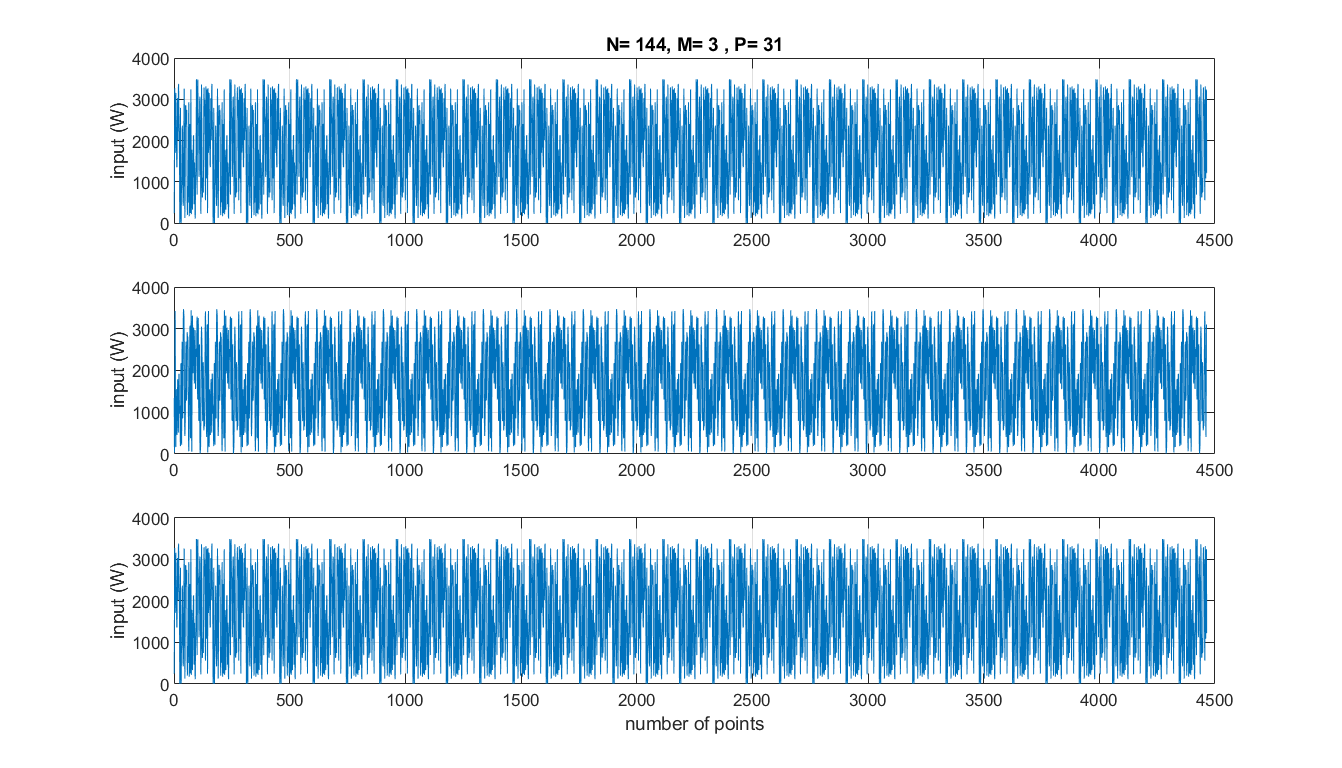
\includegraphics[width=\textwidth]{multisine.png}
    %\centering
    \caption{Input Excitation signals Robust Method}
    \label{fig:multisine}
\end{figure}

\begin{figure}[H]
    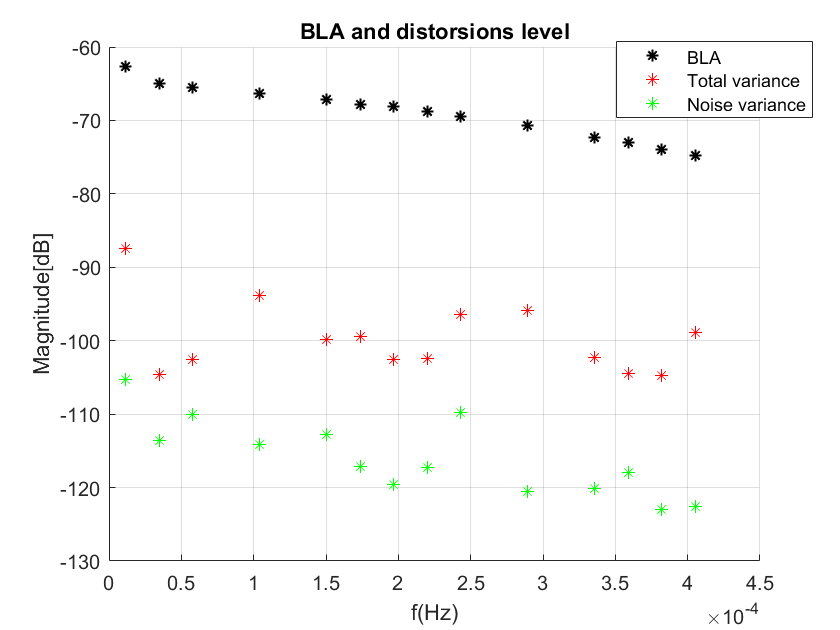
\includegraphics[width=\textwidth]{bla.png}
    %\centering
    \caption{Estimated $G_{BLA}$, total variance and noise variance}
    \label{fig:BLA}
\end{figure}

From Fig\ref{fig:BLA} we can see the excited lines in black dots.The total variance and noise variance are almost at  the same level. There is a 30dB signal to distorsion level. The variances obtained at this phase are then later on used in the parametric model Identification.A simulation was carried out to predict the output using the Non-parametric model obtained.The Input signal is a Multisine with 3 excited frequencies and RMS value of 2kW.The 3 frequency components are the first 3 bins at which the BLA was estimated.Figure \ref{fig:Npinputoutput} shows the results.

\begin{figure}[H]
    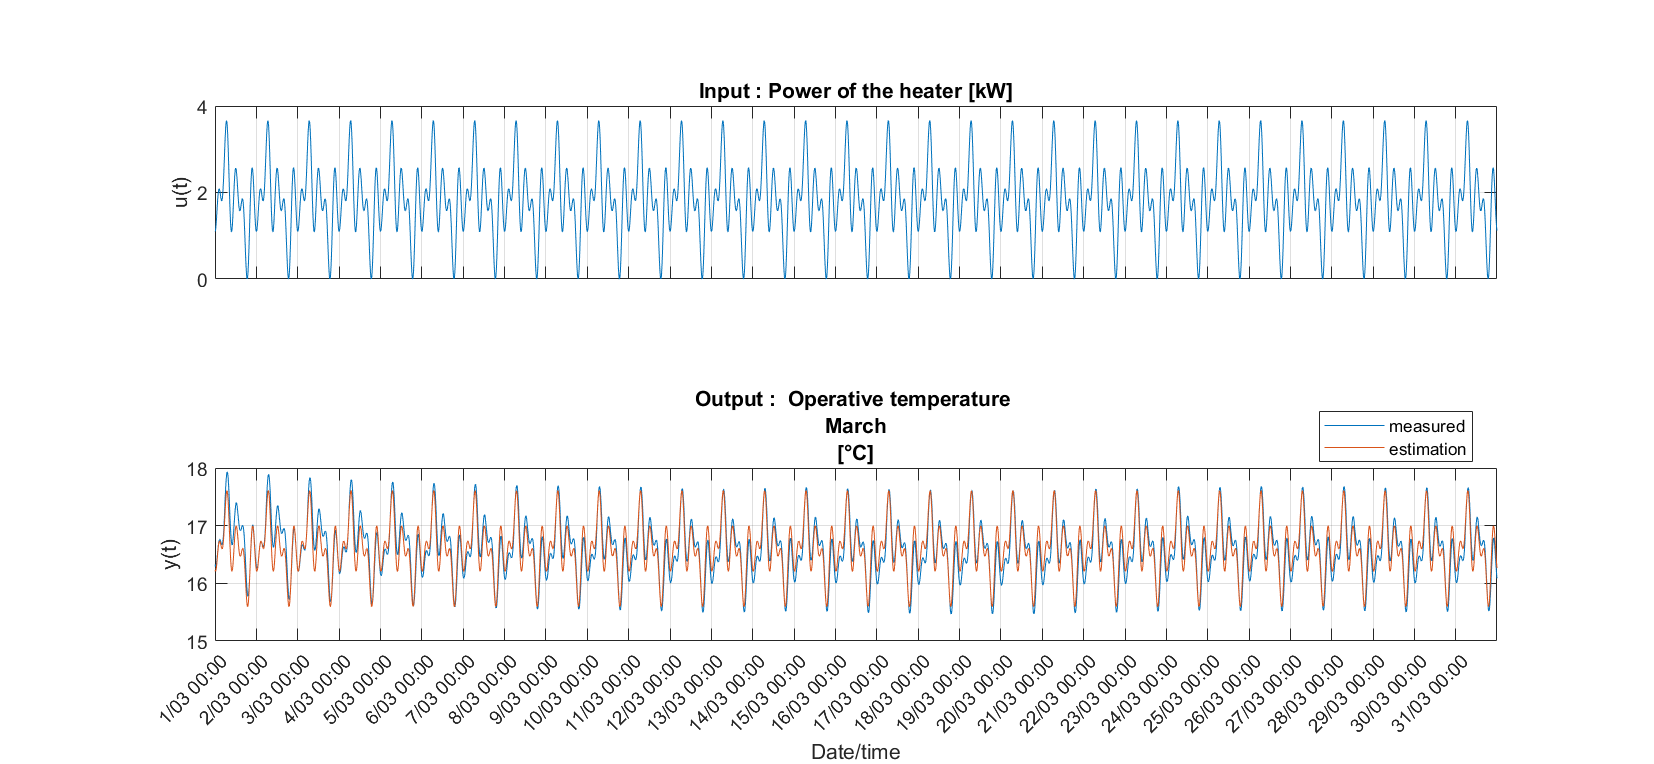
\includegraphics[width=\textwidth]{Np_In_oUT.png}
    \centering
    \caption{Non parametric model output Input output prediction}
    \label{fig:Npinputoutput}
\end{figure}

\noindent
We can see from figure \ref{fig:Npinputoutput} that the fit is not good but follows pretty well the dynamics of the system.It is a good starting point for the parametric model estimation.

\subsubsection{Estimation method parametric model}
The estimator used to obtain $G_{1}$ is the Maximum Likelihood estimator. Starting from the measured input-output DFT $U(k)$, $Y(k)$ or from a measured frequency response function $G(s_{k})$. The 2F complex-valued vector Z contains the measured
input-output (DFT) spectra , at a set of F frequencies $s_{k}$, $k = 1, 2, ...,F$
 $$
Z^{T}=\left[Z^{T}(1) Z^{T}(2) \ldots Z^{T}(F)\right] \text { with } Z^{T}(k)=[Y(k) U(k)]
$$
\noindent
we can use the output error, which is the difference between the observed output $Y(k)$ and the modeled output $Y(s_{k},\theta)$ with $\theta$ the parameter vector. For periodic signals,

\begin{equation}\label{eq:param}
Y\left(s_{k}, \theta\right)=G\left(s{k}, \theta\right) U(k)
\end{equation}

$$
G(s_{k}, \theta)=B(s_{k}, \theta) / A(s_{k}, \theta)
$$

$$
e\left(s_{k}, \theta, Z(k)\right)=A\left(s_{k}, \theta\right) Y(k)-B\left(s_{k}, \theta\right) U(k)
$$

\noindent
$e\left(s_{k}, \theta, Z(k)\right)$ is the equation error  which is the difference between the left- and right hand sides of \ref{eq:param}  after multiplication by $A\left(s_{k}, \theta\right)$.The maximum likelihood estimation consists in minimizing the  quadratic-like cost function $V_{ML}(\theta
, Z)$

\begin{equation}\label{eq:costfct}
V_{\mathrm{ML}}(\theta, Z)=\sum_{k=1}^{F} \frac{\left|e\left(s_{k}, \theta, Z(k)\right)\right|^{2}}{\sigma_{e}^{2}\left(s_{k}, \theta\right)}
\end{equation}

Dividing the numerator and denominator of each term in \ref{eq:costfct} by $\left|A\left(s_{k}, \theta\right)\right|^{2}$ gives

\begin{equation}\label{eq:costfctML}
V_{\mathrm{ML}}(\theta, Z)=\sum_{k=1}^{F} \frac{\left|Y(k)-Y\left(s_{k}, \theta\right)\right|^{2}}{\sigma_{Y}^{2}\left(s_{k}, \theta\right)}
\end{equation}

\begin{equation}
\hat{\theta}_{ML}(Z)=\arg  \min _{\theta} V_{ML}(\theta, Z)
\end{equation}


\noindent
Where $\sigma_{Y}^{2}(s_{k}, \theta)$ is the variance of the output error and $\hat{\theta}_{ML}$ the paramater vector. It is obtained from the non-parametric analysis in \ref{eq:covar} .The maximum likelihood estimator weights the equation or output error at each frequency $s_{k}$ with its measurement uncertainty, so that frequency bands with high-quality
measurements ( $\sigma_{U}^{2}(k)$ and $\sigma_{Y}^{2}(k)$ are small) contribute more to the ML (Maximum likelihood) cost than frequency bands with poor-quality measurements ( $\sigma_{U}^{2}(k)$ and $\sigma_{Y}^{2}(k)$ are large ).  Hence, in a natural way, the ML cost gives much confidence to accurate measurements while it rejects noisy measurements.

Transfer function models are not linear in the parameter and it is not possible to find and analytical solution to the optimization problem.The optimization problem is solved by iterative procedures.The minimizer $\hat{\theta}_{ML}$ will be found by a Newton-Gauss type of algorithm.By defining 

$$
\varepsilon\left(s_{k}, \theta, Z(k)\right)=\left(Y(k)-Y\left(s_{k}, \theta\right)\right) / \sigma_{Y}\left(s_{k}, \theta\right)
$$

and rewriting \ref{eq:costfctML} as $V_{ML}(\theta, Z)=\varepsilon_{\mathrm{re}}^{T}(\theta, Z) \varepsilon_{\mathrm{re}}(\theta, Z)$, where ()$_{\mathrm{re}}$ stacks the real and imaginary
parts on top of each other to obtain real parameters

$$
\varepsilon_{\mathrm{re}}(\theta, Z)=\left[\begin{array}{l}
\operatorname{Re}(\varepsilon(\theta, Z)) \\
\operatorname{Im}(\varepsilon(\theta, Z))
\end{array}\right]
$$

Each iteration calculates an increment $\Delta \theta^{(i)}=\theta^{(i)}-\theta^{(i-1)}$ given by 

$$
J_{\mathrm{re}}^{T}\left(\theta^{(i-1)}, Z\right) J_{\mathrm{re}}\left(\theta^{(i-1)}, Z\right) \Delta \theta^{(i)}=-J_{\mathrm{re}}^{T}\left(\theta^{(i-1)}, Z\right) \varepsilon_{\mathrm{re}}\left(\theta^{(i-1)}, Z\right)
$$

Where $J(\theta, Z)=\partial \varepsilon(\theta, Z) / \partial \theta$ is the Jacobian of the vector $\varepsilon(\theta, Z)$

$$
J_{\mathrm{re}}\left(\theta^{(i-1)}, Z\right) \Delta \theta^{(i)}=-\varepsilon_{\mathrm{re}}\left(\theta^{(i-1)}, Z\right)
$$

\begin{equation}\label{eq;thethaMl}
\Delta \theta^{(i)}=-J_{\mathrm{re}}\left(\theta^{(i-1)}, Z\right) \backslash \varepsilon_{\mathrm{re}}\left(\theta^{(i-1)}, Z\right)
\end{equation}


\noindent
And the new value $\theta^{(i)}=\Delta \theta^{(i)} + \theta^{(i-1)} $.The starting parameter values are obtained by linearization of the original optimization problem and to compute an analytical solution to the linearized form.This will be detailed later when discussing the Linear Least Square Estimator.The stop criterion of the iteration loop is when there is no longer a significant decrease of the cost function with iteration, then the prediction quality will not be further improved by continuing.

\paragraph{Results}
To identify the parameters of the parametric model the same input-output measurements from the non-parametric model estimation were used.The order of the transfer function was chosen from 3 model orders  by checking the quality of the fit with the non-parametric model and the stability of the model.Once a suitable order provided satisfactory results a series of check were made with new measurements to check if the fit was still of quality.

The blackbox model chosen was an Output-Error transfer function model (OE see Equation \ref{eq:trfctmodels} from chapter 4 ) whose order $n_{a}$ (order of the denominator)  and $n_{b}$
 (order of the numerator) are still to be determined. Three different model orders
were compared.The different values of  $n_{a}$ and $n_{b}$ are  presented
in table \ref{table:model order}


\begin{table}[H]
\centering
\begin{tabular}{|c|c|c|}
\hline  & n_{b} & n_{a} \\
\hline 1) & 0 & 1  \\
\hline 2) & 1 & 2  \\
\hline 3) & 2 & 3  \\
\hline
\end{tabular}
\caption{Transfer function model orders $G_{1}$}
\label{table:model order}
\end{table}

\noindent
For each model order, the Non parametric-parametric transfer function fit, pole-zero map and input-output measurements-estimation data  are presented and discussed.The simulation was done for the month of March.The Dry Bulb outside temperature was set to zero in the weather file used by EnergyPlus.Figure \ref{fig:G1mod0/1} shows the result for the first model order 0/1 ($n_{b}$/$n_{a}$)

\begin{figure}[H]
\centering
\begin{subfigure}{.5\textwidth}
  \centering
  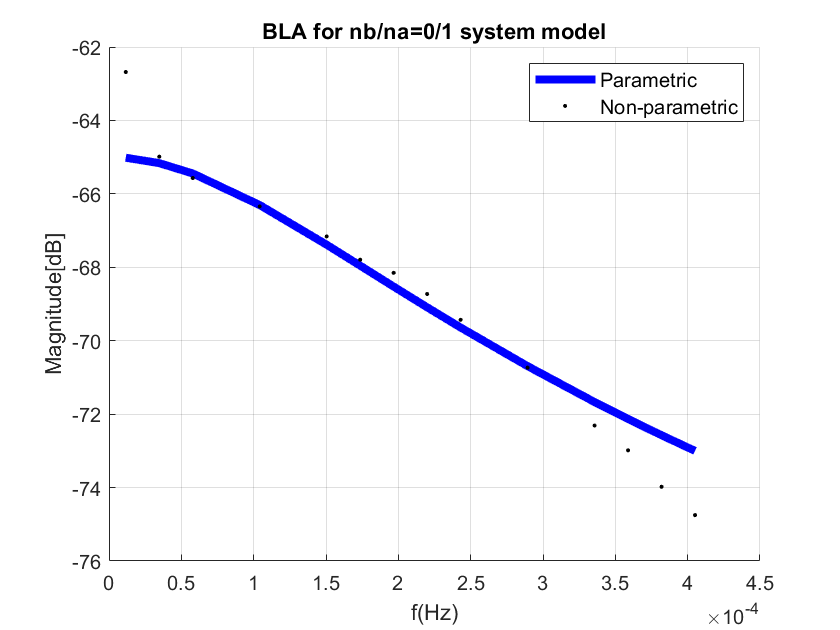
\includegraphics[width=.7\linewidth]{G1mod01FrfFit.png}
  \caption{FRF fit}
  \label{fig:frf fit G1mod0/1}
\end{subfigure}%
\begin{subfigure}{.5\textwidth}
  \centering
  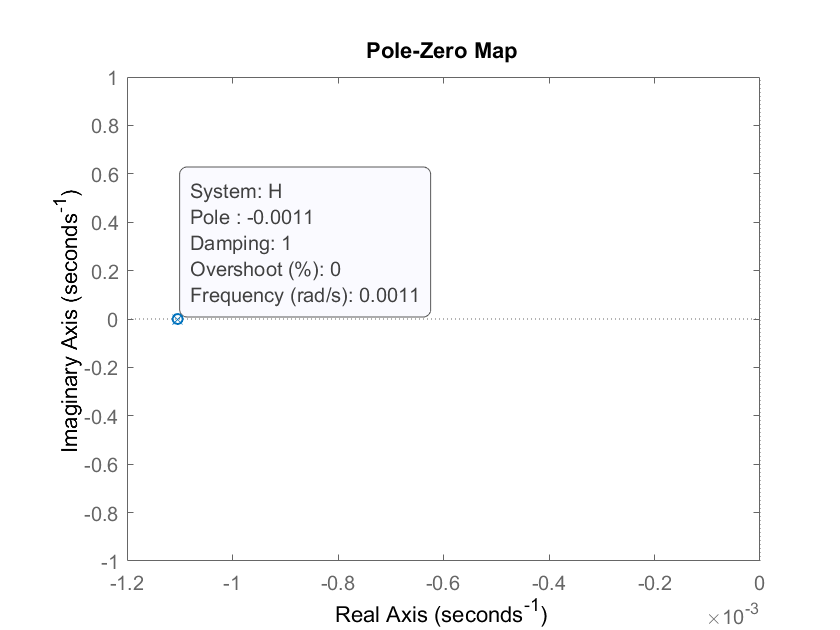
\includegraphics[width=.7\linewidth]{G1mod01pzmap.png}
  \caption{pole-zero map}
  \label{fig:pzmap G1mod0/1}
\end{subfigure}

\begin{subfigure}{\textwidth}
  \centering
  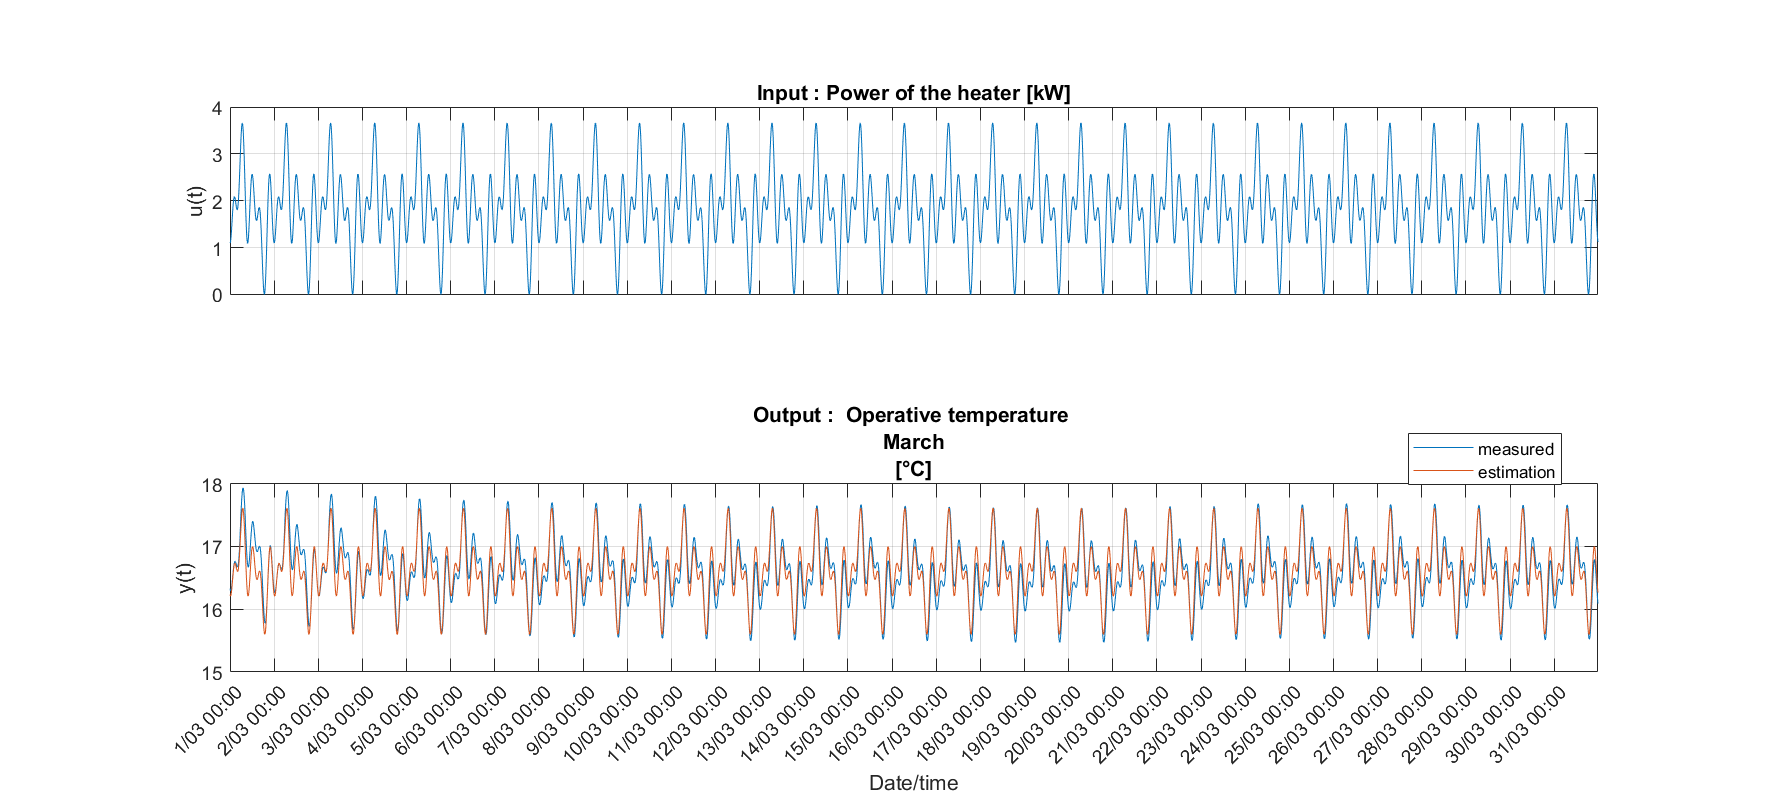
\includegraphics[scale=0.38]{G1mod01InOut.png}
  \caption{Measured and Estimated outputs}
  \label{fig:inoutG10/1}
\end{subfigure}
\caption{Results $G_{1}$ Identification with a model order of 0/1 }
\label{fig:G1mod0/1}
\end{figure}

\noindent
From figure \ref{fig:inoutG10/1} we can see that the fit is not good.The model is able to predict some of the dynamics of the system but without a good accuracy. From figure \ref{fig:frf fit G1mod0/1} we can see that the fit is not good in the lower and upper end of the excited band.This yields a model that is too simple.From figure \ref{fig:pzmap G1mod0/1} we can see that the pole obtained is stable and is in the excited band.The second model order was analysed next.Figure \ref{fig:G1mod1/2} shows the results for the second model order 1/2 

\begin{figure}[H]
\centering
\begin{subfigure}{.5\textwidth}
  \centering
  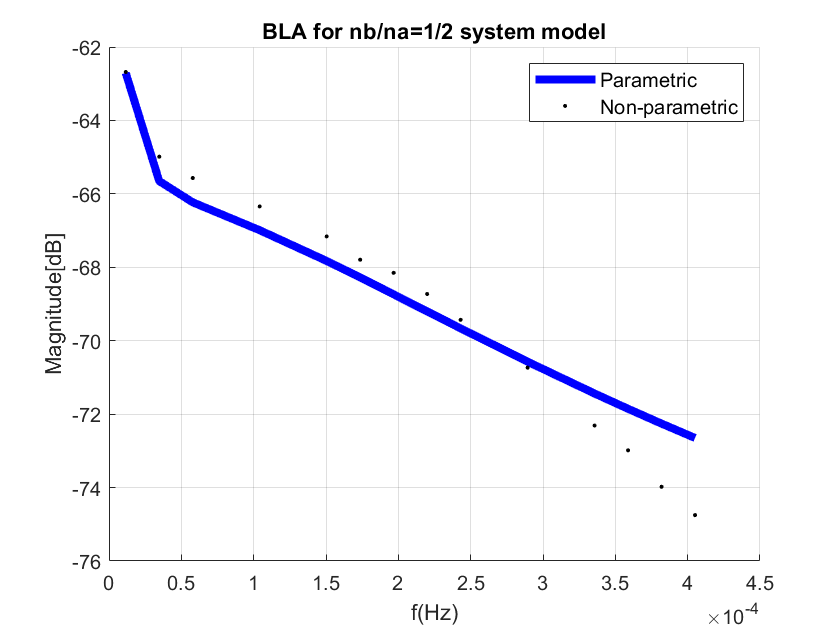
\includegraphics[width=.7\linewidth]{G1mod12FrfFit.png}
  \caption{FRF fit}
  \label{fig:frf fit G1mod1/2}
\end{subfigure}%
\begin{subfigure}{.5\textwidth}
  \centering
  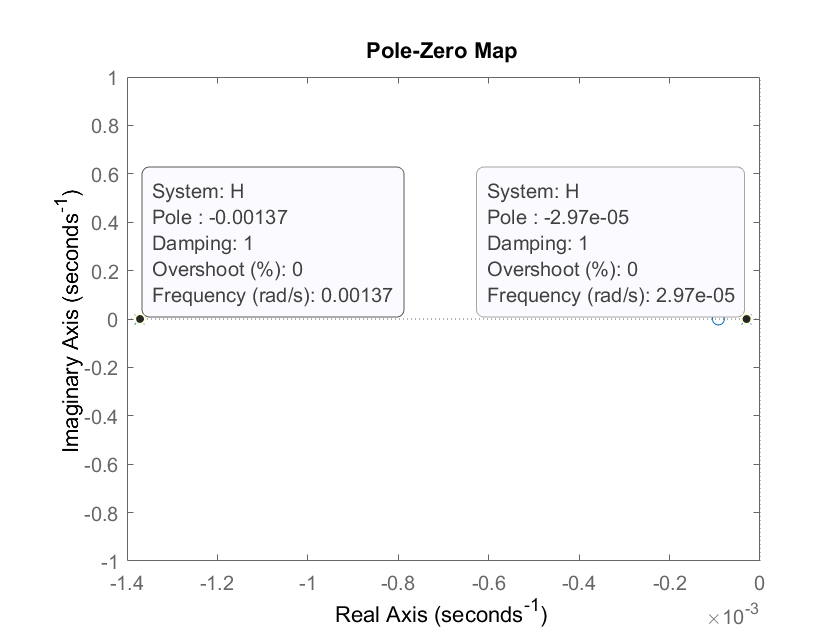
\includegraphics[width=.7\linewidth]{G1mod12pzmap.png}
  \caption{pole-zero map}
  \label{fig:pzmap G1mod1/2}
\end{subfigure}

\begin{subfigure}{\textwidth}
  \centering
  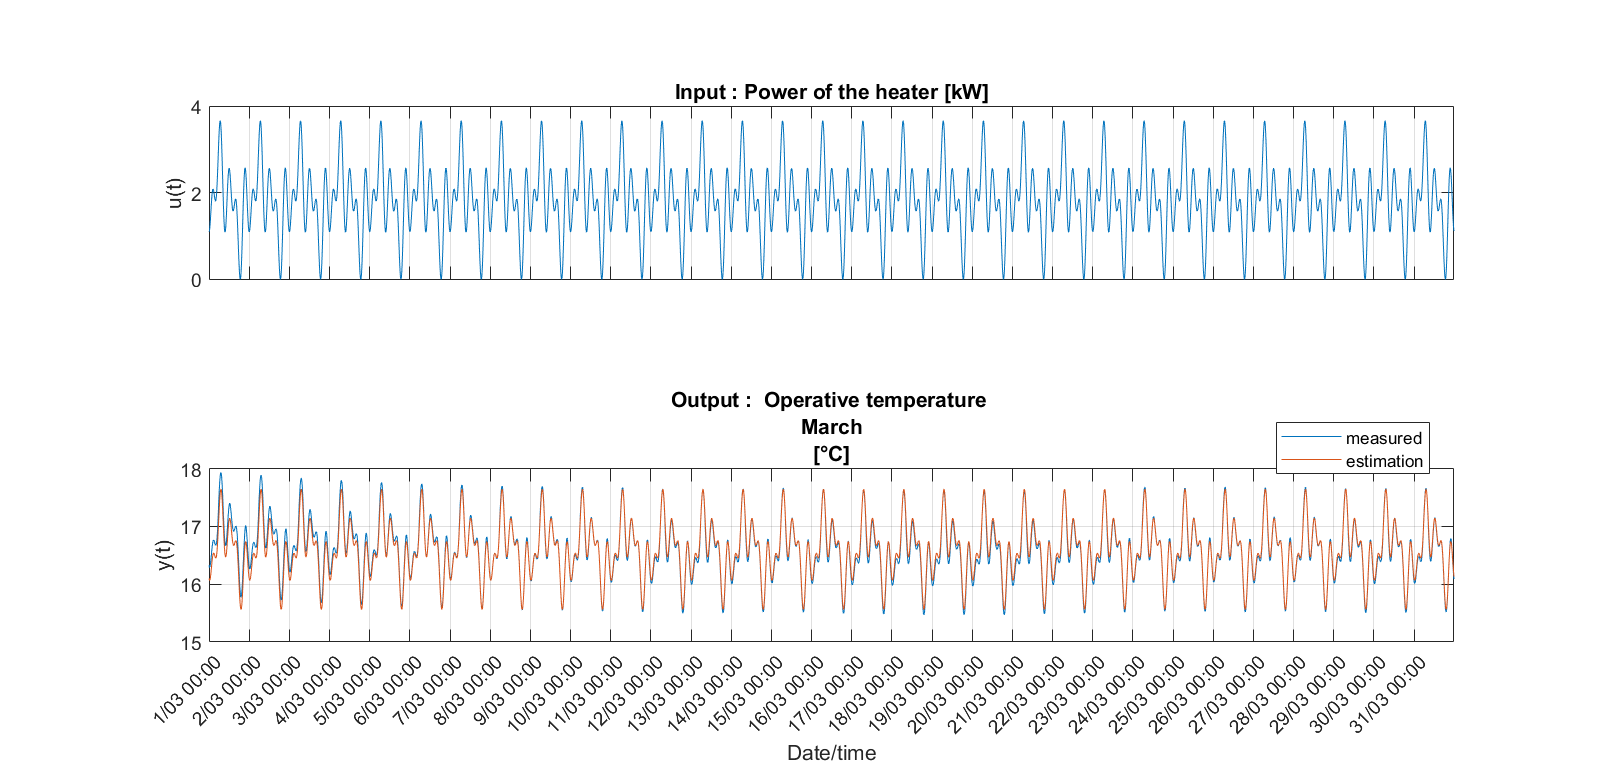
\includegraphics[scale=0.38]{G1mod12InOut.png}
  \caption{Measured and Estimated outputs}
  \label{fig:inoutG11/2}
\end{subfigure}
\caption{Results $G_{1}$ Identification with a model order of 1/2 }
\label{fig:G1mod1/2}
\end{figure}

\noindent
From figure \ref{fig:inoutG11/2} we can see that we have a good fit.Steady state is reached after around 4 days.From day1 to day4 we are in a transient state and the fit is not good.From day7 to day14 the fit is very good and from day15 to day22 the fit is good and it seems as if there is a periodic disturbance of period 7 days. From figure \ref{fig:frf fit G1mod1/2} we can see that the fit is good in the lower band than the previous fit.This yields a good model as the dynamics of the system are in the lowest frequency band.From figure \ref{fig:pzmap G1mod1/2} we can see that the poles obtained are stable and are in the excited band.The third model order was analysed next.Figure \ref{fig:G1mod2/3} shows the results for the third model order 2/3 


\begin{figure}[H]
\centering
\begin{subfigure}{.5\textwidth}
  \centering
  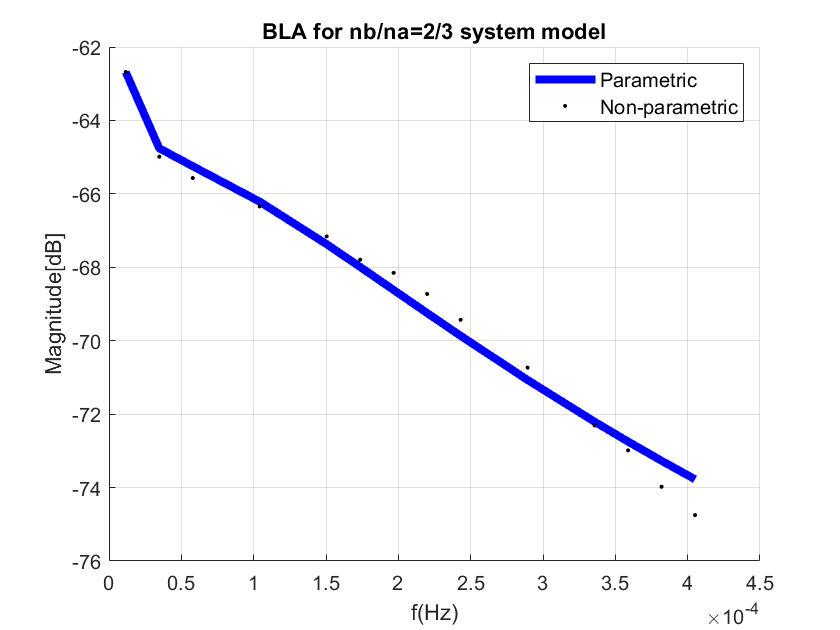
\includegraphics[width=.7\linewidth]{G1mod23FrfFit.png}
  \caption{FRF fit}
  \label{fig:frf fit G1mod2/3}
\end{subfigure}%
\begin{subfigure}{.5\textwidth}
  \centering
  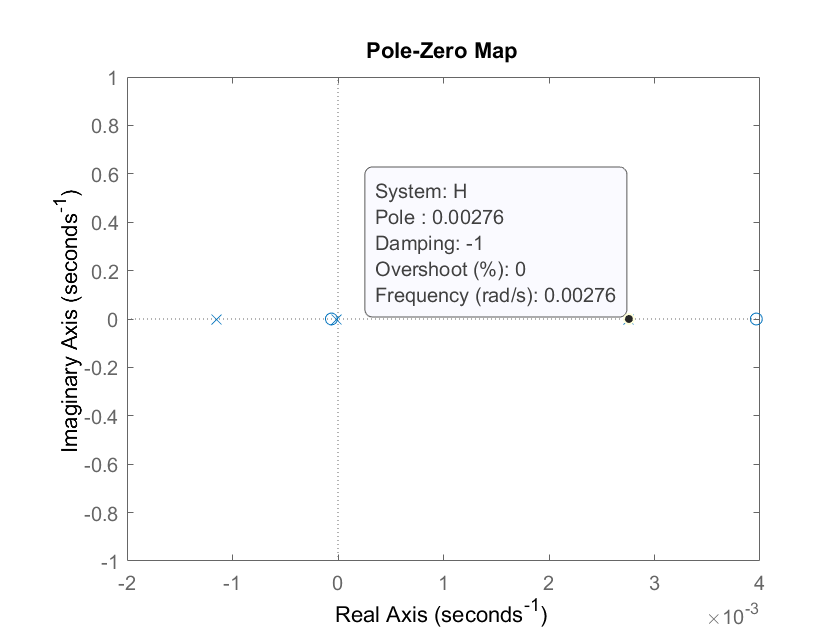
\includegraphics[width=.7\linewidth]{G1mod23pzmap.png}
  \caption{pole-zero map}
  \label{fig:pzmap G1mod2/3}
\end{subfigure}

\begin{subfigure}{\textwidth}
  \centering
  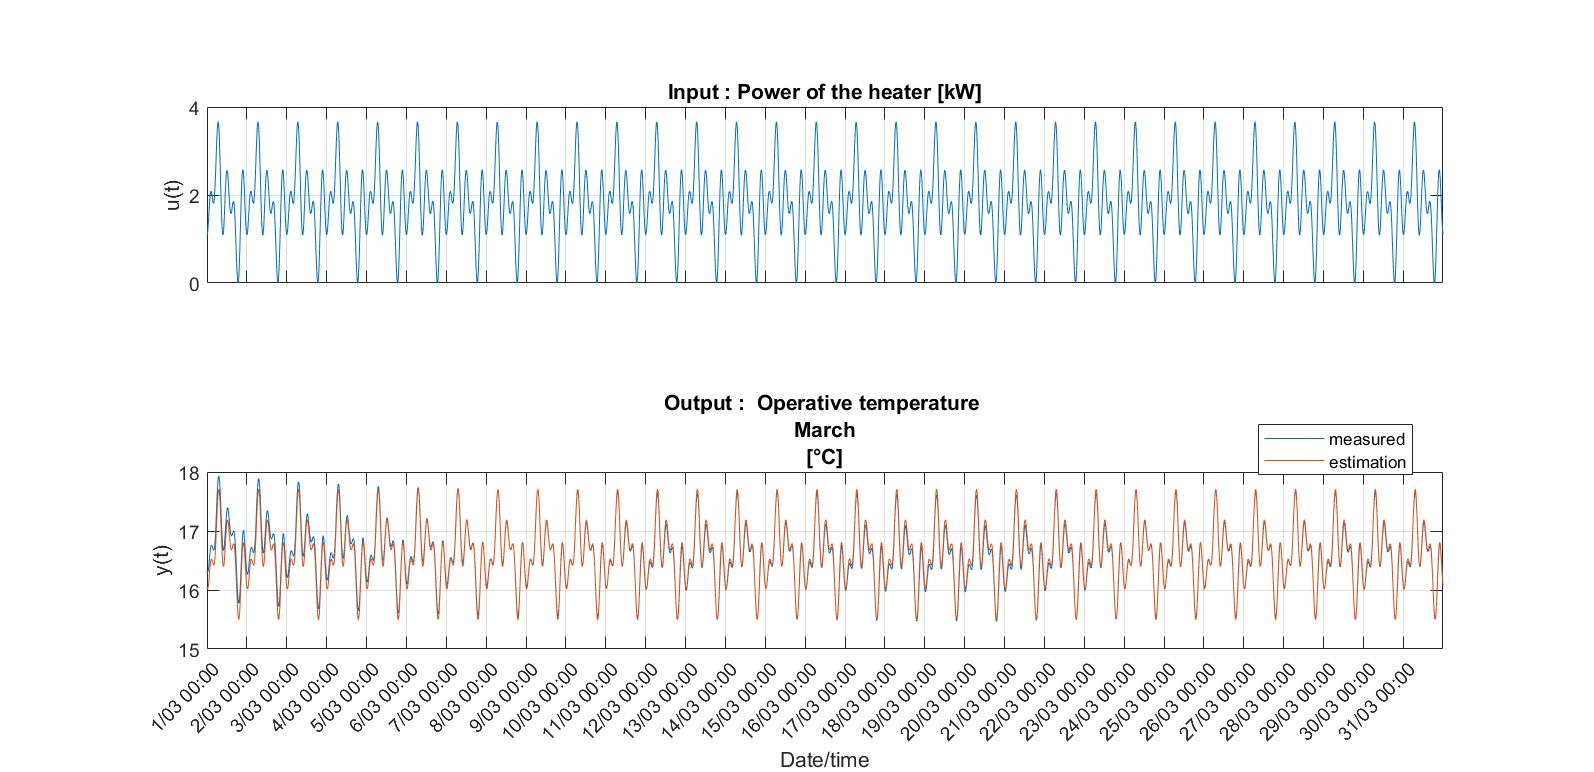
\includegraphics[scale=0.38]{G1mod23InOut.png}
  \caption{Measured and Estimated outputs}
  \label{fig:inoutG12/3}
\end{subfigure}
\caption{Results $G_{1}$ Identification with a model order of 2/3 }
\label{fig:G1mod2/3}
\end{figure}

\noindent
From figure \ref{fig:inoutG12/3} we can see that the fit is as good as with the 1/2 model.From figure \ref{fig:pzmap G1mod2/3} we can see that one of the pole obtained is unstable and is outside of the excited band.This indicates that the model is too complex.From figure \ref{fig:frf fit G1mod2/3} we can see that the fit is better in the lower band and upper end of the excited band.Despite the improvement of the fit, the prediction accuracy did not improve and indicates that the non improvement of the fit is not due to modelling errors.The final model order chosen was the 1/2 model as it had a good FRF and output prediction fit and had stable poles.

The second step was to do a cross validation check with new data set to validate the model obtained.Three  experiments were carried out, a first simulation with one day of data with input multisine signal,a second one with one day of data with input an arbitrary signal and a last one with one month of data with multisine input signal.The multisines's frequencies were all in the excitation band of the estimation.The Dry Bulb outside temperature was set to zero in the weather file used by EnergyPlus. Figure \ref{fig:G1onedayValidation15/07}shows the results of the model validation for one day of data.The simulation was done on the 15th of July with as input a multisine with an RMS value of 2kW.

\begin{figure}[H]
    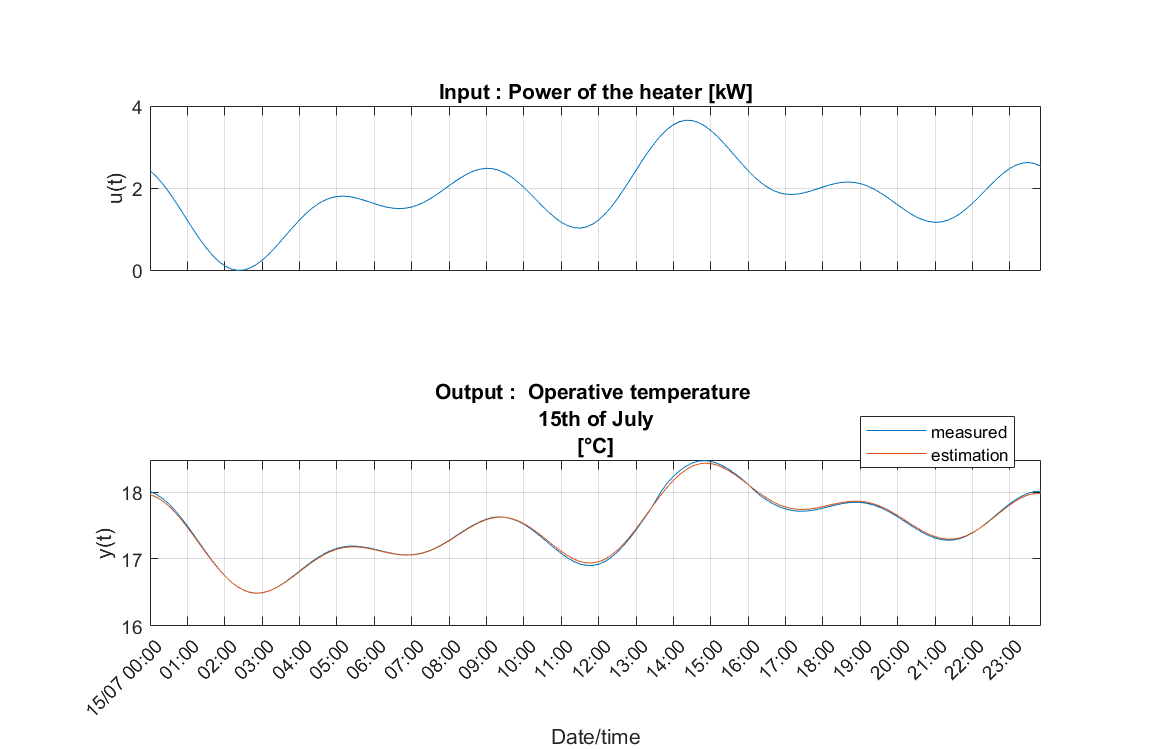
\includegraphics[width=\textwidth]{G1_15_07_MS.png}
    \centering
    \caption{$G_{1}$ validation model 15th of July multisine Result}
    \label{fig:G1onedayValidation15/07}
\end{figure}

\noindent
We can see from Figure \ref{fig:G1onedayValidation15/07} that the fit is good.The model is able to predict outputs with new data from another month different of the estimation month.The second experiment was also done on the 15th of July with an arbitary input excitation signal with an RMS value of 2.5kW. Figure \ref{fig:G1onedayValidation15/07Ran} shows the results obtained.

\begin{figure}[H]
    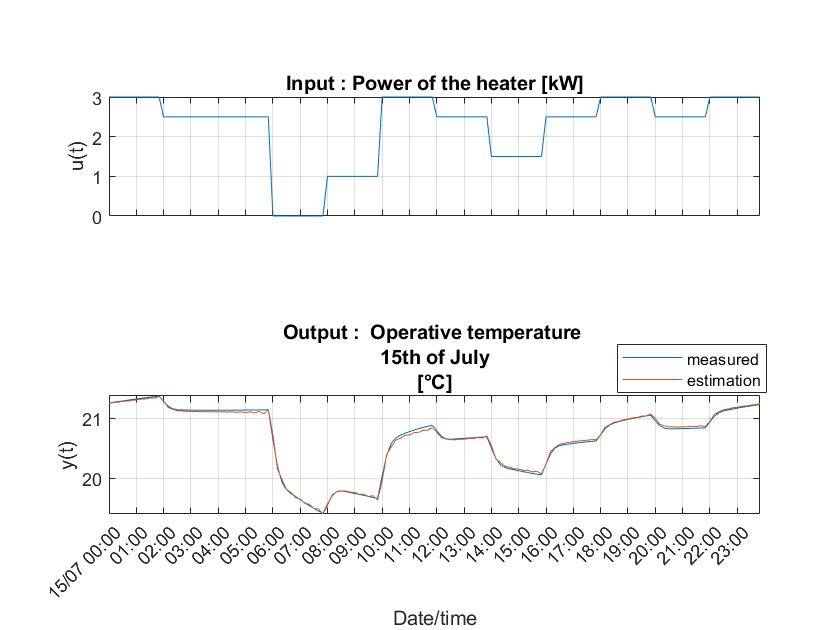
\includegraphics[width=\textwidth]{G1_15_07_RanIn.png}
    \centering
    \caption{$G_{1}$ validation model 15th of July arbitrary Result}
    \label{fig:G1onedayValidation15/07Ran}
\end{figure}

\noindent
We can see from Figure \ref{fig:G1onedayValidation15/07Ran} that the fit is good.The model is able to predict outputs with new data with an input of different class than the one used for the estimation.The Last experiment was  done on the month of November with a Multisine input excitation signal with an RMS value of 2kW. Figure \ref{fig:G1onedayValidationNov} shows the results obtained.

\begin{figure}[H]
    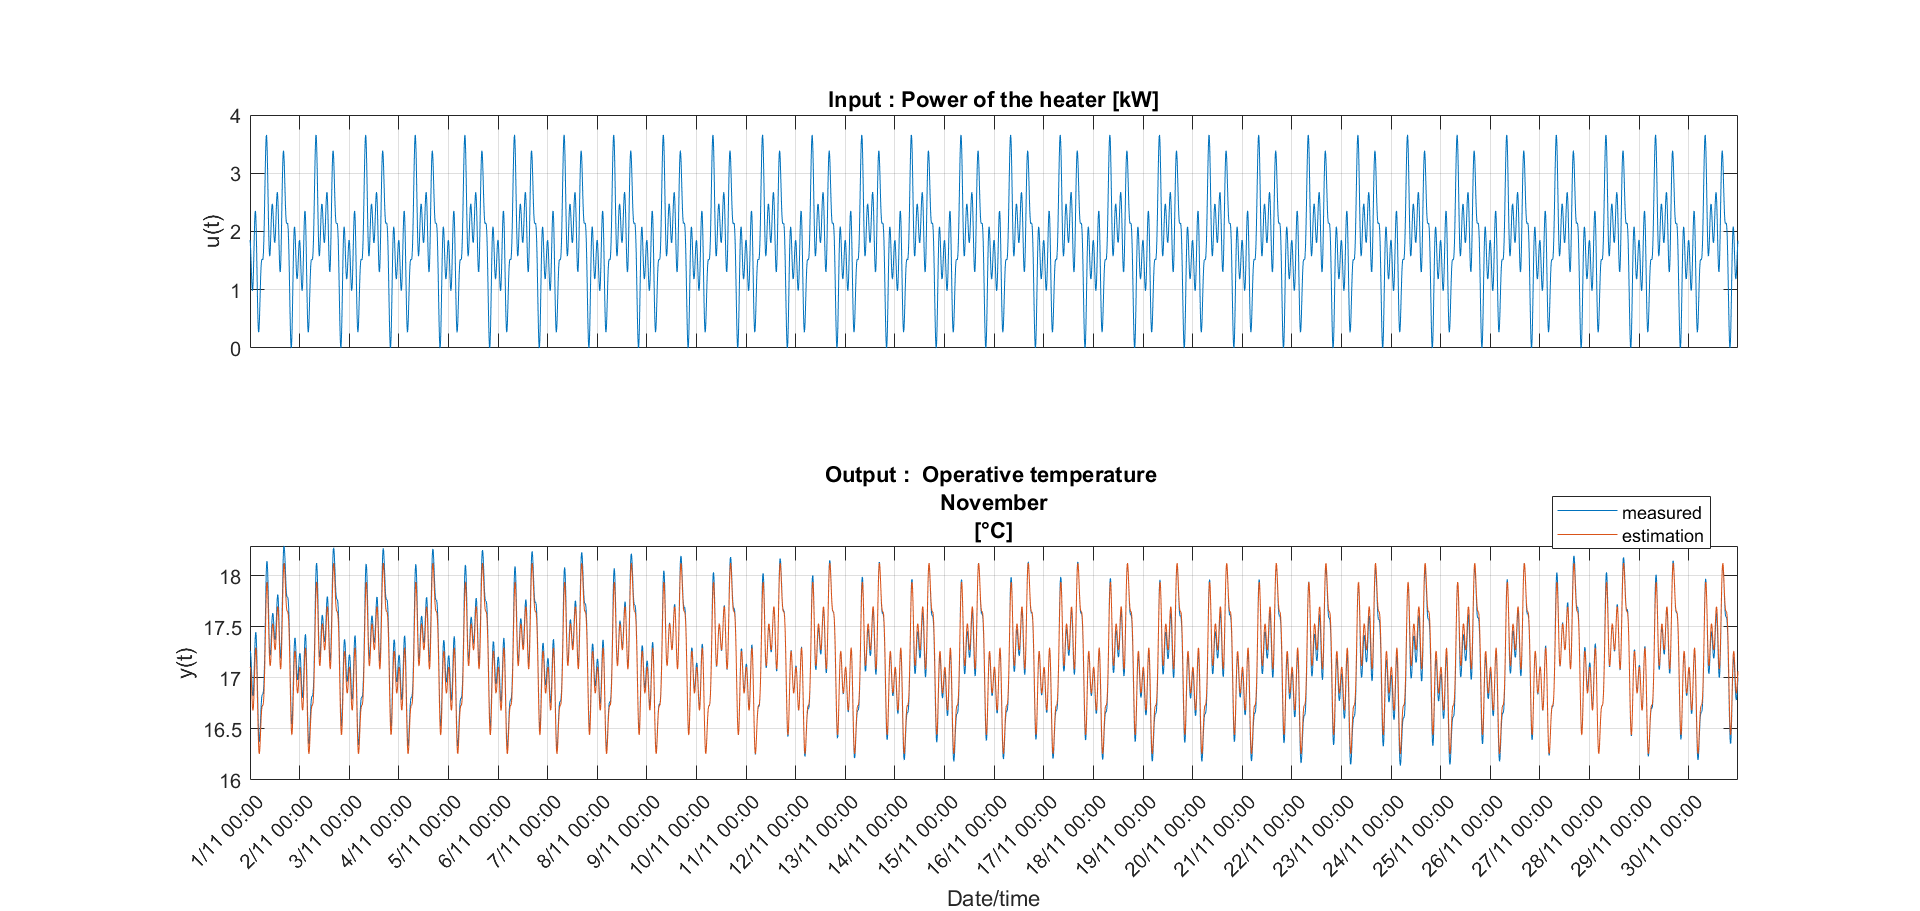
\includegraphics[width=\textwidth]{G1_val_NOV.png}
    \centering
    \caption{$G_{1}$ validation model month of November  Result}
    \label{fig:G1onedayValidationNov}
\end{figure}

\noindent
We can see from Figure \ref{fig:G1onedayValidationNov} that the fit is good.The model is able to predict outputs with new data and different month than the estimation month.The identification of the Heater model $G_{1}$ gave satisfactory results.The next step is the identification of the Dry Bulb to operative temperature $G_{2}$.

\subsection{Identification of Dry Bulb Model G2 }
Due to the nature of the excitation signal; the dry bulb outside temperature, the parametric model $G_{2}$ was obtained directly that is there was no non-parametric model estimated in a first step.

\subsubsection{Excitation design}
The dry bulb temperature being a non uncontrollable input,typical measurements value were obtained from a weather file.The robust method is to be used with sinusoidal input signal that is why a non-parametric model was not estimated.Usually to estimate the FRF multiple experiments are made and averaging techniques are then used to estimate the FRF.With data from the weather file only a single experiment could be made.

\subsubsection{Model structure}
The aim of the model is for control purposes.The choice is the same as for the $G_{1}$ model a continuous time parametric black-box model.More precisely an ARMAX transfer function whose whose order $n_{a}$,$n_{b}$ and order of the transient term $n_{i}$ are to be determined.The ARMAX transfer function  is of the form

\begin{equation}
\begin{aligned}
Y(s_{k}) &=G(s_{k}, \theta) U(k)+T^{\circ}(s_{k}, \theta) \\
&=\frac{B(s_{k}, \theta)}{A(s_{k}, \theta)} U(k)+\frac{I(s_{k}, \theta)}{A(s_{k}, \theta)}
\end{aligned}
\end{equation}

\subsubsection{Estimation method}
The estimator used to obtain $G_{2}$ is the linear least square estimator. Starting from the measured input-output DFT $U(k)$, $Y(k)$ or from a measured frequency response function $G(s_{k})$. The 2F complex-valued vector Z contains the measured
input-output (DFT) spectra , at a set of F frequencies $s_{k}$, $k = 1, 2, ...,F$
 $$
Z^{T}=\left[Z^{T}(1) Z^{T}(2) \ldots Z^{T}(F)\right] \text { with } Z^{T}(k)=[Y(k) U(k)]
$$
\noindent
 For arbitrary signals,the input-output relationship is of the form

\begin{equation}\label{eq:armax}
Y\left(s_{k}, \theta\right)=G\left(s{k}, \theta\right) U(k) + T_{G}\left(s_{k}, \theta\right)
\end{equation}

$$
G(s_{k}, \theta)=B(s_{k}, \theta) / A(s_{k}, \theta)
$$

$$
e\left(s_{k}, \theta, Z(k)\right)=A\left(s_{k}, \theta\right) Y(k)-B\left(s_{k}, \theta\right) U(k)- I\left(s_{k}, \theta\right)
$$
\noindent
$e\left(s_{k}, \theta, Z(k)\right)$ is the equation error  which is the difference between the left- and right hand sides of \ref{eq:armax}  after multiplication by $A\left(s_{k}, \theta\right)$.The linear least square estimation consists in minimizing the  quadratic-like cost function $V_{LS}(\theta
, Z)$

\begin{equation}\label{eq:Levy}
V_{\mathrm{LS}}(\theta, Z)=\sum_{k=1}^{F}\left|e\left(s_{k}, \theta, Z(k)\right)\right|^{2}
\end{equation}

\noindent
For numerical purposes,we impose that $a_{0}$=1.This method was proposed by Levy.The drawback of this method is the the overemphasizing of high-frequency errors in \ref{eq:Levy}.Indeed, the term $A\left(s_{k}, \theta\right)$ has bigger values at high frequencies than at low frequencies and this result in poor low-frequency fits.A refined linearization method was proposed by Sanathanan.To obtain a better fit at low frequencies as well as at
high frequencies, he proposes to approximate the denominator $A\left(s_{k}, \theta\right)$ in some parameter-independent way. The denominator at iteration $i$ is approximated by its expression at iteration $i-1$.

\begin{equation}
V_{LS}\left(Z, \theta^{(i)}\right)=\sum_{k=1}^{F}\left|\frac{A\left(s_{k}, \theta^{(i)}\right) Y_{m}(k)-B\left(s_{k}, \theta^{(i)}\right) U(k)-I\left(s_{k}, \theta^{(i)}\right)}{A\left(s_{k}, \hat{\theta}^{(i-1)}\right)}\right|^{2}
\end{equation}

\noindent
The initial estimate used at iteration $i$=1 is obtained with the Levy estimation method.The estimate is of the same form as \ref{eq;thethaMl} (see Appendix for more details of the computation)

\begin{equation}\label{eq:ThethaSanathanan}
\Delta \theta^{(i)}=-J_{\mathrm{san}}\left(\theta^{(i-1)}, Z\right) \backslash \varepsilon_{\mathrm{san}}\left(\theta^{(i-1)}, Z\right)
\end{equation}

\paragraph{Results}
The estimation was done with input data from a wzeather file and output data from EnergyPlus.The order of the transfer function was chosen from 3 model orders by checking the quality of the fit estimated and measured output and the stability of the model.Once a suitable order provided satisfactory results, series of check were made with new measurements to see if the prediction was still accurate.

\noindent
Three different model orders were compared.The different values of  $n_{a}$,$n_{b}$ and $n_{i}$ are  presented in table \ref{table:model order G_{2}}

\begin{table}[H]
\centering
\begin{tabular}{|c|c|c|c|}
\hline  & n_{b} & n_{a} & n_{i} \\
\hline 1) & 0 & 1 & 2 \\
\hline 2) & 1 & 2 & 3\\
\hline 3) & 2 & 3 & 4\\
\hline
\end{tabular}
\caption{Transfer function model orders $G_{2}$}
\label{table:model order G_{2}}
\end{table}

\noindent
For each model order, the pole-zero map and input-output measurements-estimation data  are presented and discussed.The simulation was done for the month of February.The Heater power was set to zero in EnergyPlus.Figure \ref{fig:G2mod0/1} shows the result for the first model order 0/1 ($n_{b}$/$n_{a}$) and $n_{i}$=2

\begin{figure}[H]
\centering
\begin{subfigure}{.5\textwidth}
  \centering
  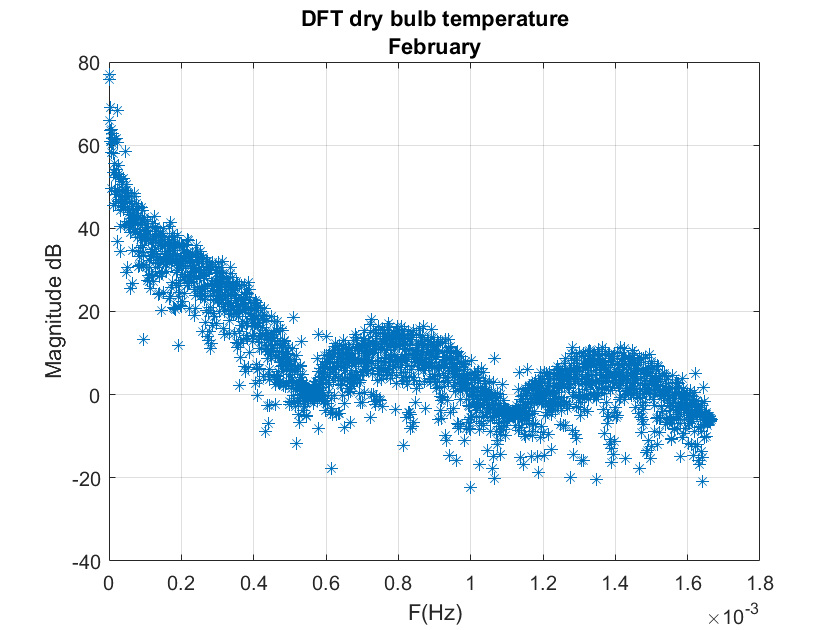
\includegraphics[width=.7\linewidth]{Dft_drybulbFeb.png}
  \caption{DFT dry bulb temperature month of February}
  \label{fig:DFT G2mod0/1}
\end{subfigure}%
\begin{subfigure}{.5\textwidth}
  \centering
  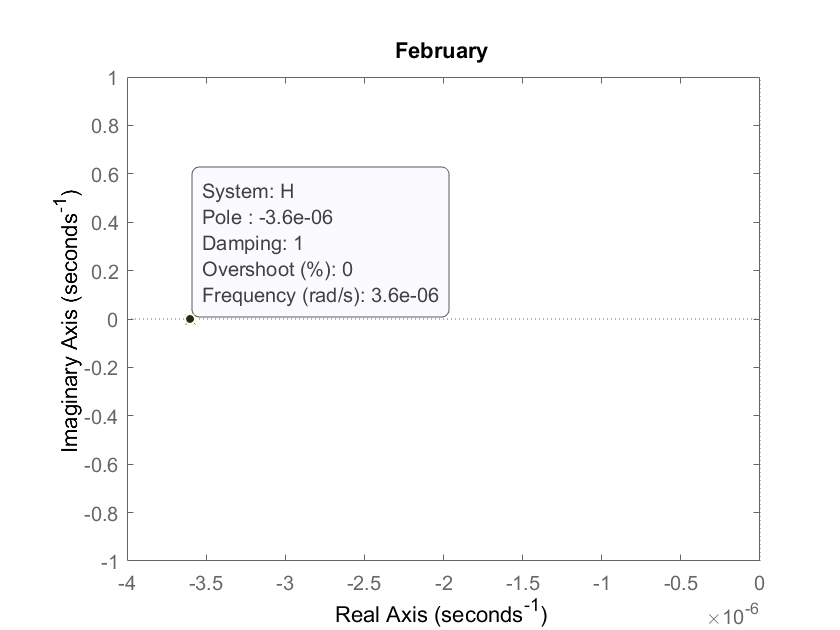
\includegraphics[width=.7\linewidth]{G2mod01pzmap.png}
  \caption{pole-zero map}
  \label{fig:pzmap G2mod0/1}
\end{subfigure}

\begin{subfigure}{\textwidth}
  \centering
  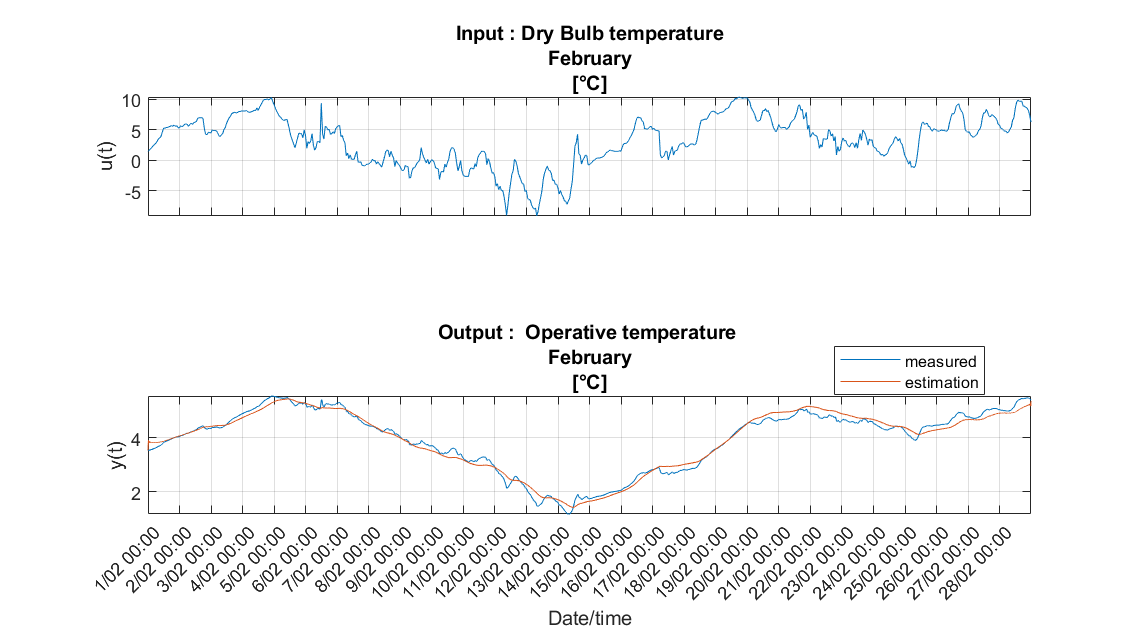
\includegraphics[scale=0.38]{G2mod01InOut.png}
  \caption{Measured and Estimated outputs}
  \label{fig:inoutG20/1}
\end{subfigure}
\caption{Results $G_{1}$ Identification with a model order of 0/1 and $n_{i}$=2}
\label{fig:G2mod0/1}
\end{figure}

\noindent
From figure \ref{fig:inoutG20/1} we can see that the fit is not good.The model is able to follow the dynamics of the system but lacks accuracy. From figure \ref{fig:DFT G2mod0/1} we can see that the excited band is from $0-1,67.10^{-3}\;Hz$/ $0.010\;rad/s$.From figure \ref{fig:pzmap G2mod0/1} we can see that the pole obtained is stable and is in the excited band.The second model order was analysed next.Figure \ref{fig:G2mod1/2} shows the results for the second model order 1/2 and and $n_{i}$=3

\begin{figure}[H]
\centering
\begin{subfigure}{.5\textwidth}
  \centering
  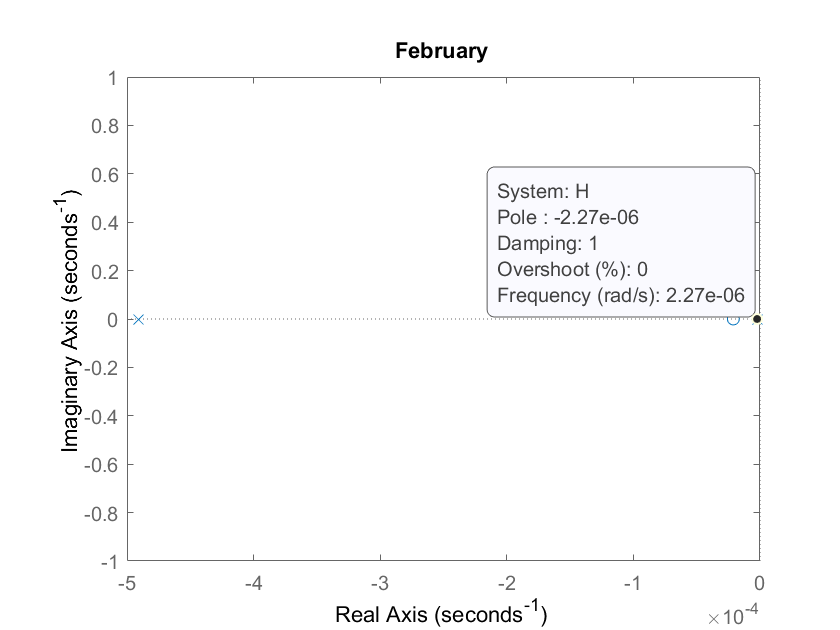
\includegraphics[width=.7\linewidth]{G2mod12pzmap.png}
  \caption{pole-zero map}
  \label{fig:pzmap G2mod1/2}
\end{subfigure}

\begin{subfigure}{\textwidth}
  \centering
  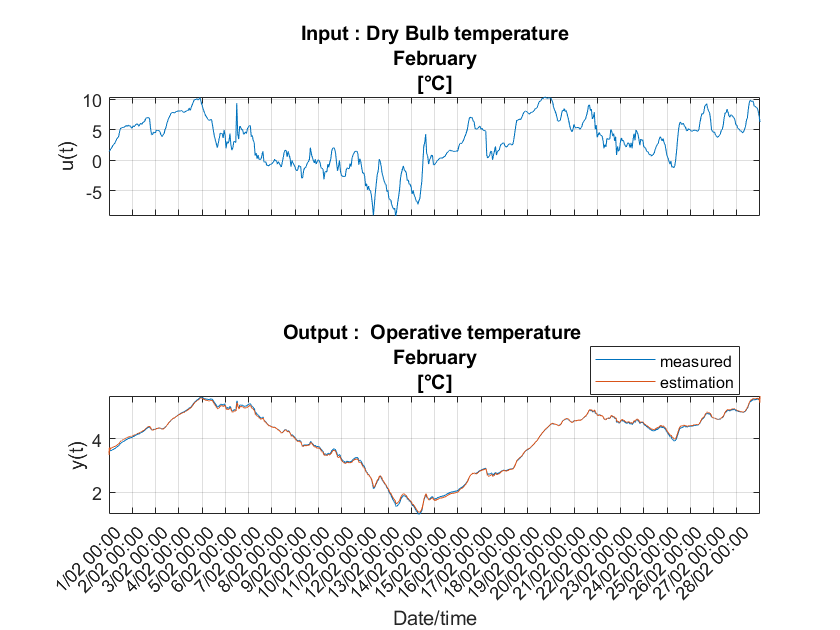
\includegraphics[scale=0.38]{G2mod12InOut.png}
  \caption{Measured and Estimated outputs}
  \label{fig:inoutG21/2}
\end{subfigure}
\caption{Results $G_{2}$ Identification with a model order of 1/2 $n_{i}$=3 }
\label{fig:G2mod1/2}
\end{figure}

\noindent
From figure \ref{fig:inoutG21/2} we can see that we have a good fit.We can see that the fit is good from the beginning of the month.This is because the transient was also estimated.From figure \ref{fig:pzmap G2mod1/2} we can see that the poles obtained are stable and are in the excited band.The third model order was analysed next.Figure \ref{fig:G2mod2/3} shows the results for the third model order 2/3 and $n_{i}$=4

\begin{figure}[H]
\centering
\begin{subfigure}{.5\textwidth}
  \centering
  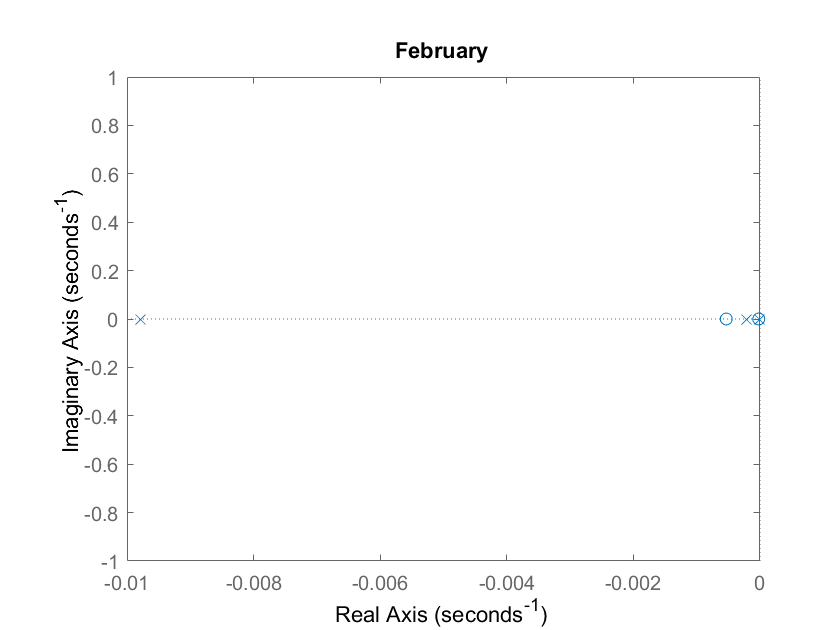
\includegraphics[width=.7\linewidth]{G2mod23pzmap.png}
  \caption{pole-zero map}
  \label{fig:pzmap G2mod2/3}
\end{subfigure}

\begin{subfigure}{\textwidth}
  \centering
  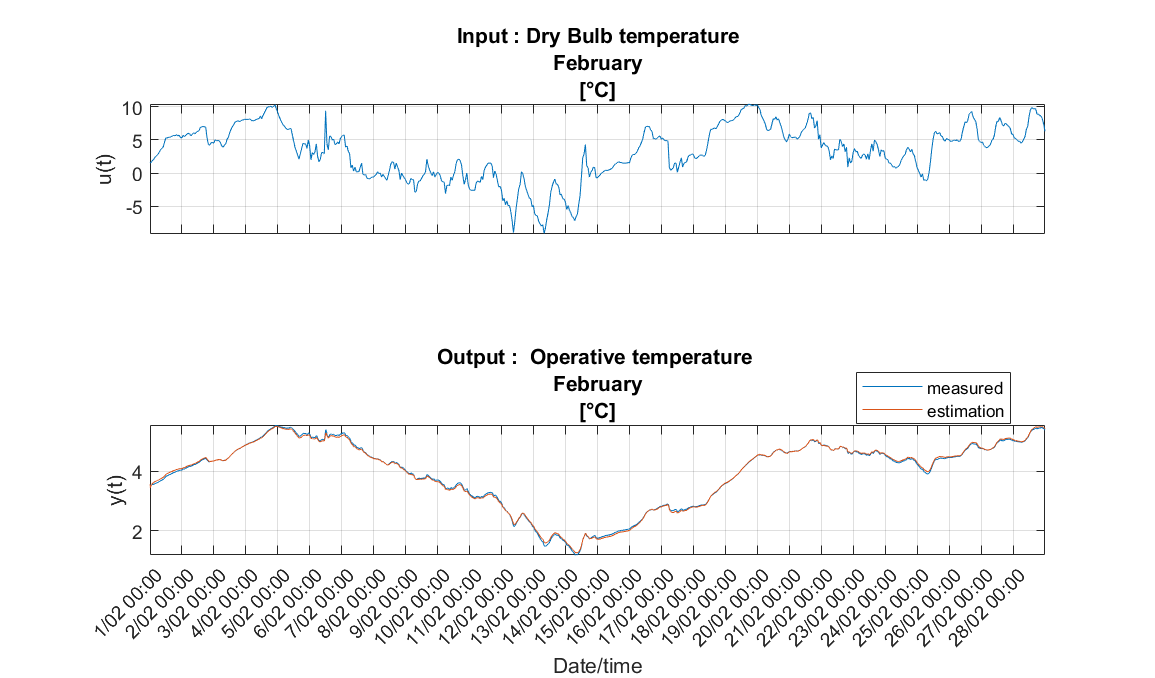
\includegraphics[scale=0.38]{G2mod23InOut.png}
  \caption{Measured and Estimated outputs}
  \label{fig:inoutG22/3}
\end{subfigure}
\caption{Results $G_{2}$ Identification with a model order of 2/3 and $n_{i}$=4 }
\label{fig:G2mod2/3}
\end{figure}

\noindent
From figure \ref{fig:inoutG22/3} we can see that the fit is as good as with the 1/2 model.From figure \ref{fig:pzmap G2mod2/3} we can see that there is a pole/zero cancellation.This indicates that the perfect fit has been reached and further increasing the model order will not improve the fit.The final model order chosen was the 1/2 model as it had a good  output prediction fit and had stable poles.

The second step was to do a cross validation check with new data set to validate the model obtained.Two  experiments were carried out, a first simulation with one day of data and a second one with one month of data .The heater power was set to zero in  EnergyPlus. Figure \ref{fig:G2onedayValidation10/07}shows the results of the model validation for one day of data.The simulation was done on the 10th of July with as input the dry bulb temperature of the 10th of July obtained from the weather file..No transient term with data set from the month of July was estimated.

\begin{figure}[H]
    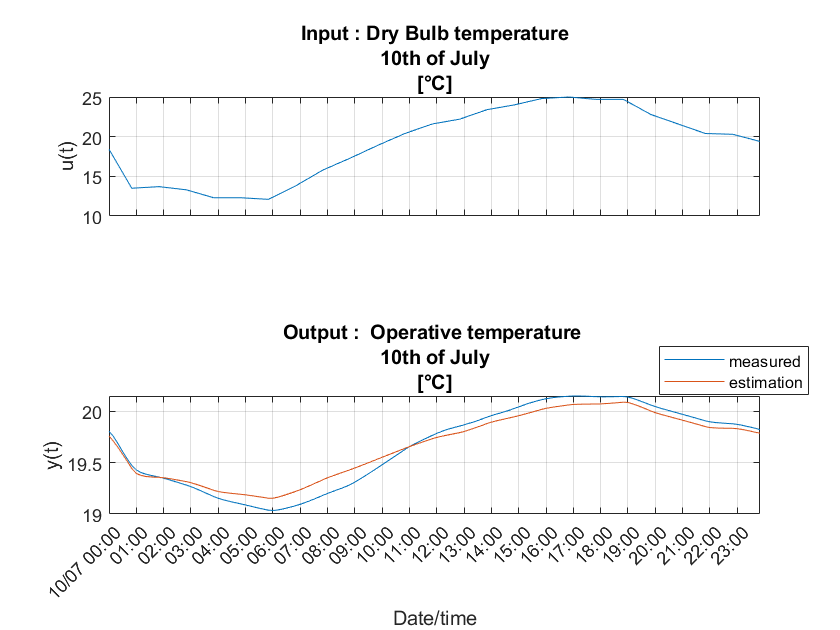
\includegraphics[width=\textwidth]{G2_10_07.png}
    \centering
    \caption{$G_{2}$ validation model 10th of July  Result}
    \label{fig:G2onedayValidation10/07}
\end{figure}

\noindent
From  figure \ref{fig:G2onedayValidation10/07} we can see that the fit is acceptable.The model obtained with data from the month of February is able to follow the dynamics with data from the month of July.The second experiment was  done on the month of October with input the dry bulb temperature of the month of October obtained from the weather file. Figure \ref{fig:G2oneMONTHValidation} shows the results obtained.No transient term with data set from the month of October was estimated.

\begin{figure}[H]
    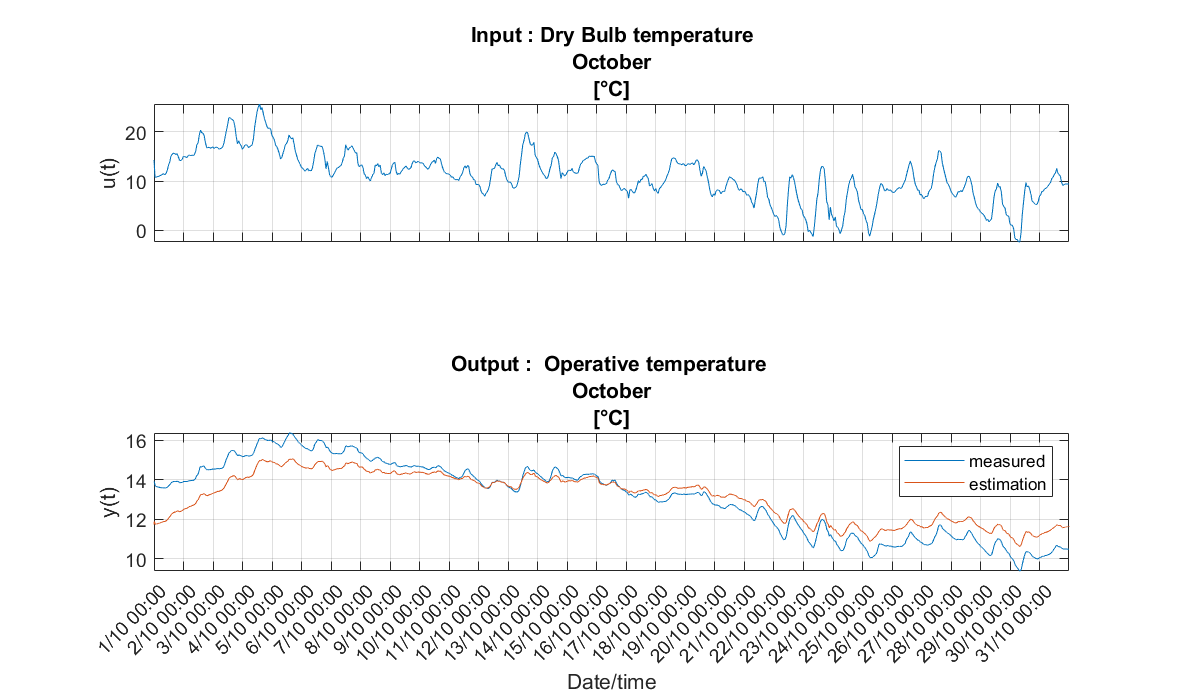
\includegraphics[width=\textwidth]{G2_val_OCT.png}
    \centering
    \caption{$G_{2}$ validation model month of October Result}
    \label{fig:G2oneMONTHValidation}
\end{figure}

From  figure \ref{fig:G2oneMONTHValidation} we can see that the fit is not good.The model obtained with data from the month of February is not able to give a good prediction for all the other months.A $G_{2}$ model has to be estimated for each month.Figure \ref{fig:G2othermonth} shows the results obtained when a  $G_{2}$ model is estimated with data from that month.The transient term was also estimated.

\begin{figure}[H]
\centering
\begin{subfigure}{.5\textwidth}
  \centering
  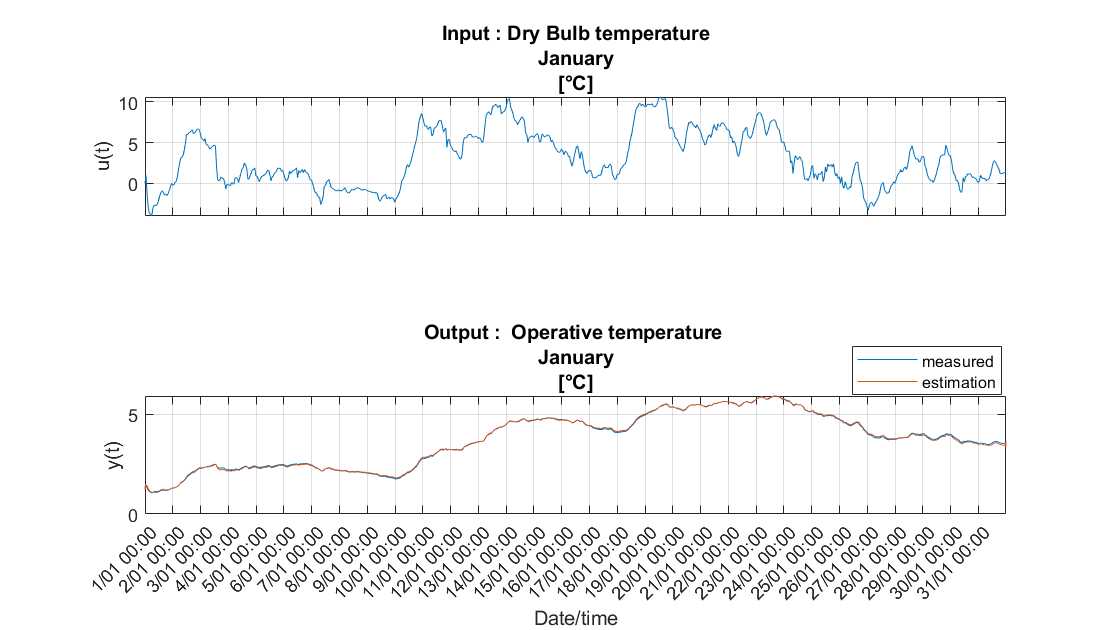
\includegraphics[width=.7\linewidth]{G2_Jan.png}
  \caption{$G_{2}$ model January}
  \label{fig:G2 Jan}
\end{subfigure}%
\begin{subfigure}{.5\textwidth}
  \centering
  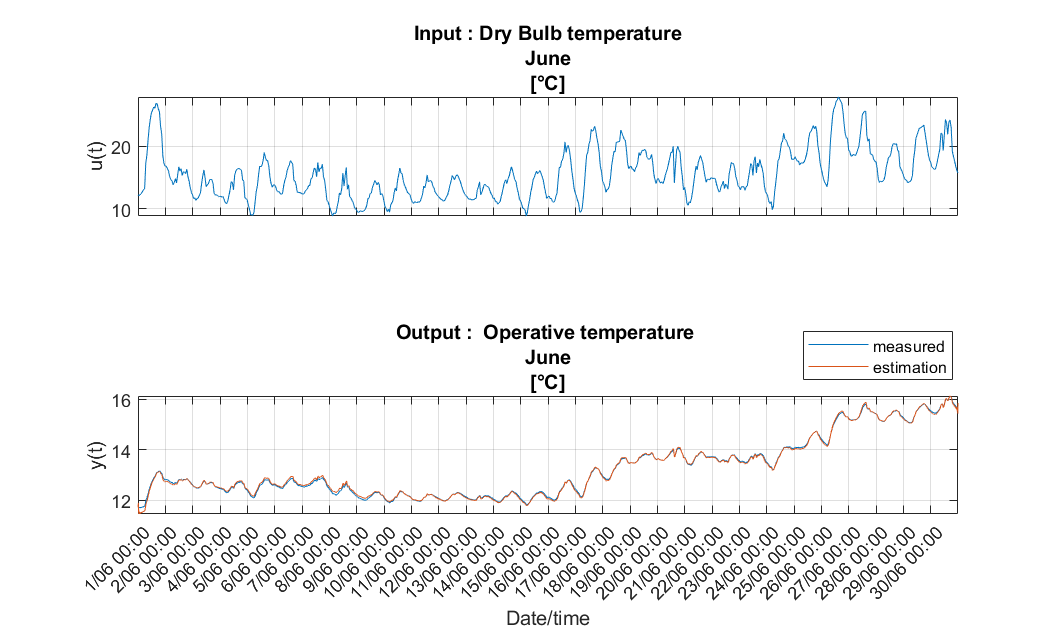
\includegraphics[width=.7\linewidth]{G2_June.png}
  \caption{$G_{2}$ model June}
  \label{fig:G2 June}
\end{subfigure}

\begin{subfigure}{\textwidth}
  \centering
  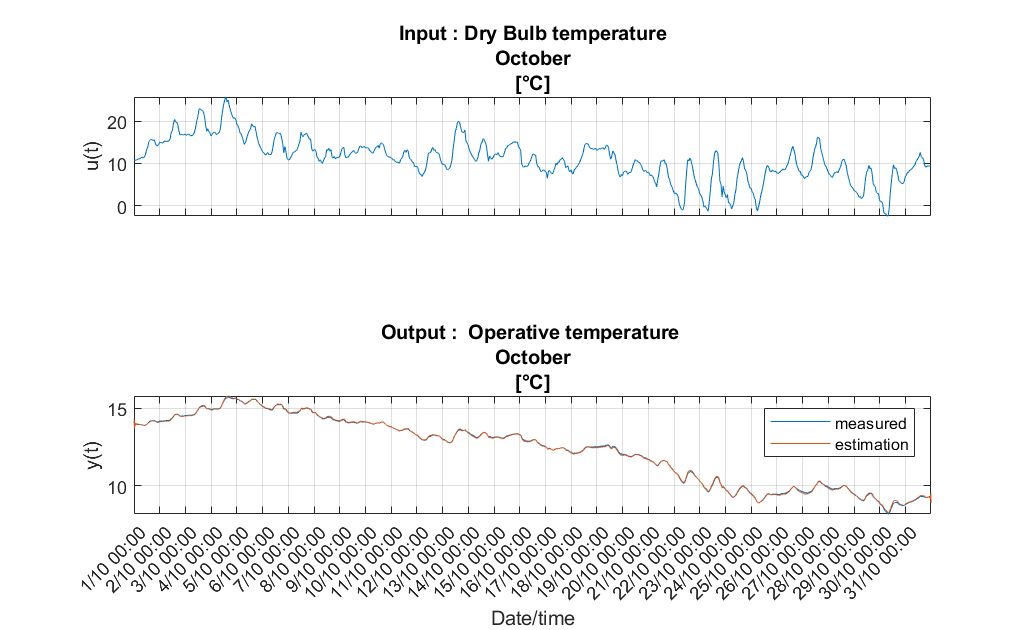
\includegraphics[scale=0.38]{G2_Oct.png}
  \caption{$G_{2}$ model October}
  \label{fig:G2 october}
\end{subfigure}
\caption{Results $G_{2}$ with data from that month}
\label{fig:G2othermonth}
\end{figure}

\subsection{Parameterization of coefficients of G2 models}
In the previous section it was seen that a $G_{2}$ model estimated with data from a particular month will not do a good prediction if used to predict the output for a different month.It happens that the poles and zeroes of the models obtained from each month are close.Figure\ref{fig:pzmapmanymonths} shows the pole-zero map for different months.

\begin{figure}[H]
\centering
\begin{subfigure}{.5\textwidth}
  \centering
  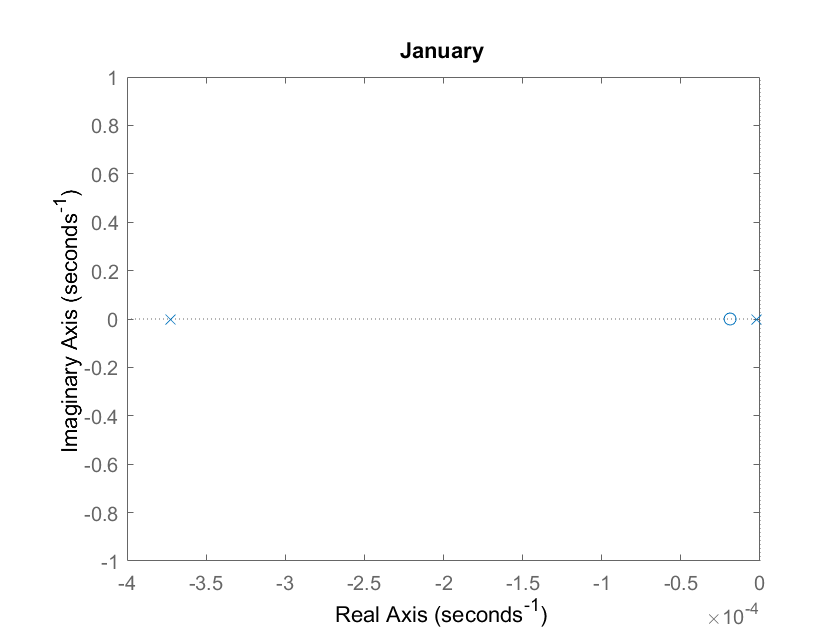
\includegraphics[width=.7\linewidth]{G2_jan_pzmap.png}
  \caption{$G_{2}$ January pole-zero map}
  \label{fig:G2_jan_pzmap}
\end{subfigure}%
\begin{subfigure}{.5\textwidth}
  \centering
  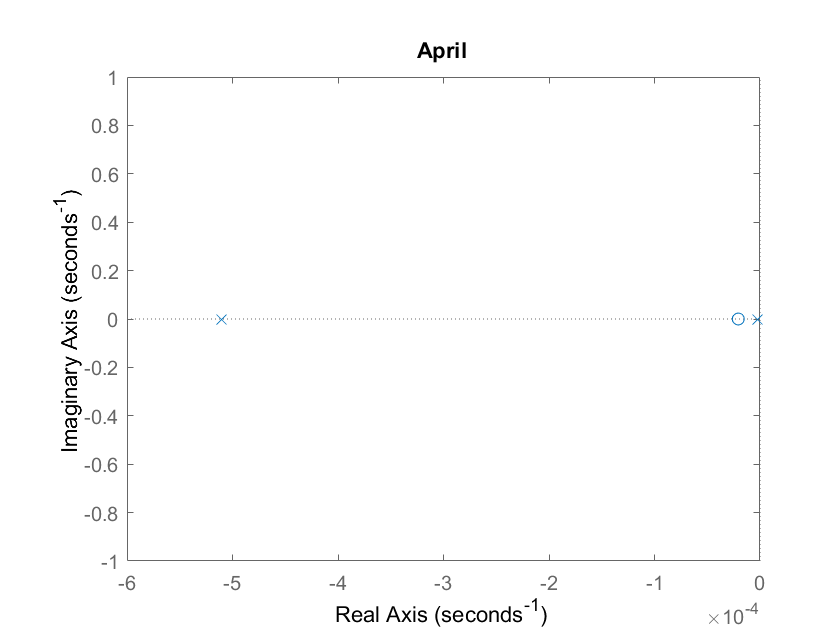
\includegraphics[width=.7\linewidth]{G2_apr_pzmap.png}
  \caption{$G_{2}$ model April pole-zero map}
  \label{fig:G2_apr_pzmap}
\end{subfigure}
\begin{subfigure}{.5\textwidth}
  \centering
  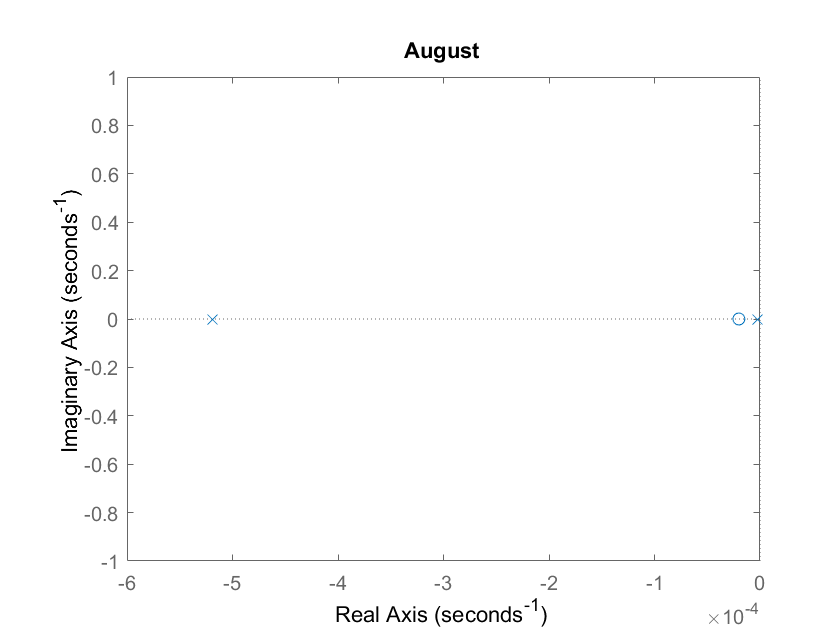
\includegraphics[width=.7\linewidth]{G2_aug_pzmap.png}
  \caption{$G_{2}$ model August pole-zero map}
  \label{fig:G2_aug_pzmap}
\end{subfigure}%
\begin{subfigure}{.5\textwidth}
  \centering
  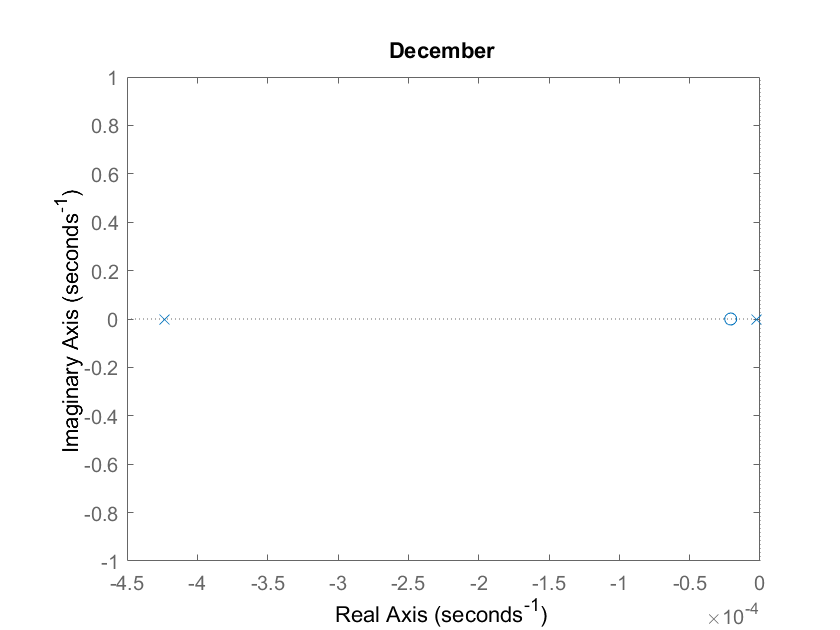
\includegraphics[width=.7\linewidth]{G2_dec_pzmap.png}
  \caption{$G_{2}$ model December pole-zero map}
  \label{fig:G2_dec_pzmap}
\end{subfigure}
\caption{pole-zero maps $G_{2}$ with data from the corresponding month}
\label{fig:pzmapmanymonths}
\end{figure}

A bode diagram of the 12 months can also be viewed from figure\ref{fig;bodeG2}.We can see that the transfer functions are alike.

\begin{figure}[H]
    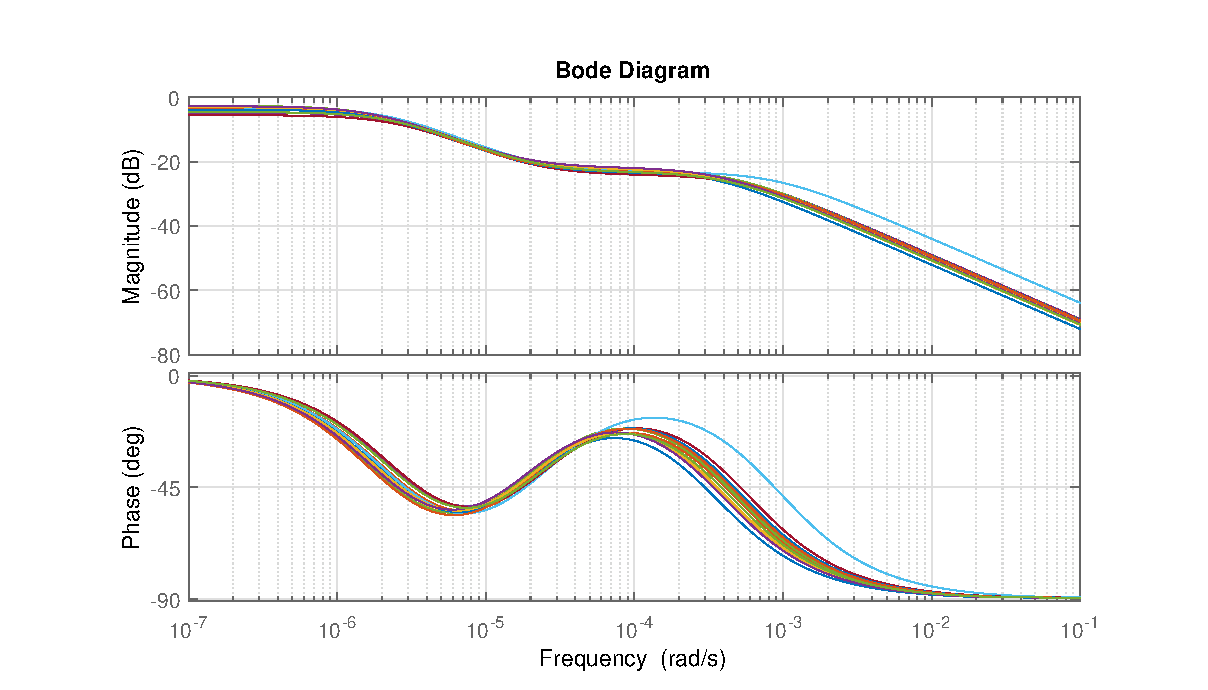
\includegraphics[width=\textwidth]{Bode_plot_Jan_Dec.eps}
    \centering
    \caption{Bode plot 12 months}
    \label{fig;bodeG2}
\end{figure}


\subsubsection{Method}
The method consists of carrying out 12 identification procedures to determine the coefficients $n_{a}$ and $n_{b}$ of $G_{2}$ for each month.Then a quadratic curve is fitted to each of the coefficients by cubic spline interpolation. Cubic spline interpolation is the process of constructing a spline $f:\left[x_{1}, x_{n+1}\right] \rightarrow \mathbb{R}$ which consists of $n$ polynomials of degree three, referred to as $f_{1}$ to $f_{n}$. A spline is a function defined by piecewise polynomials.The  interpolation function traverses all $n+1$ points.The resulting function has the following structure:

$$
f(x)= \begin{cases}a_{1} x^{3}+b_{1} x^{2}+c_{1} x+d_{1} & \text { if } x \in\left[x_{1}, x_{2}\right] \\ a_{2} x^{3}+b_{2} x^{2}+c_{2} x+d_{2} & \text { if } x \in\left(x_{2}, x_{3}\right] \\ \cdots & \\ a_{n} x^{3}+b_{n} x^{2}+c_{n} x+d_{n} & \text { if } x \in\left(x_{n}, x_{n+1}\right]\end{cases}
$$

\noindent
Where $x$ is the index of the month considered and coefficients $a_{i}$, $b_{i}$, $c_{i}$ and $d_{i}$ are to be determined(see appendix for more details).

\subsubsection{Results}
Figure\ref{fig:fitcurves} shows the fitted curve obtained for each coefficient.The model order is a 1/2 model.The cubic spline interpolation fits nicely the data.

\begin{figure}[H]
\centering
\begin{subfigure}{.5\textwidth}
  \centering
  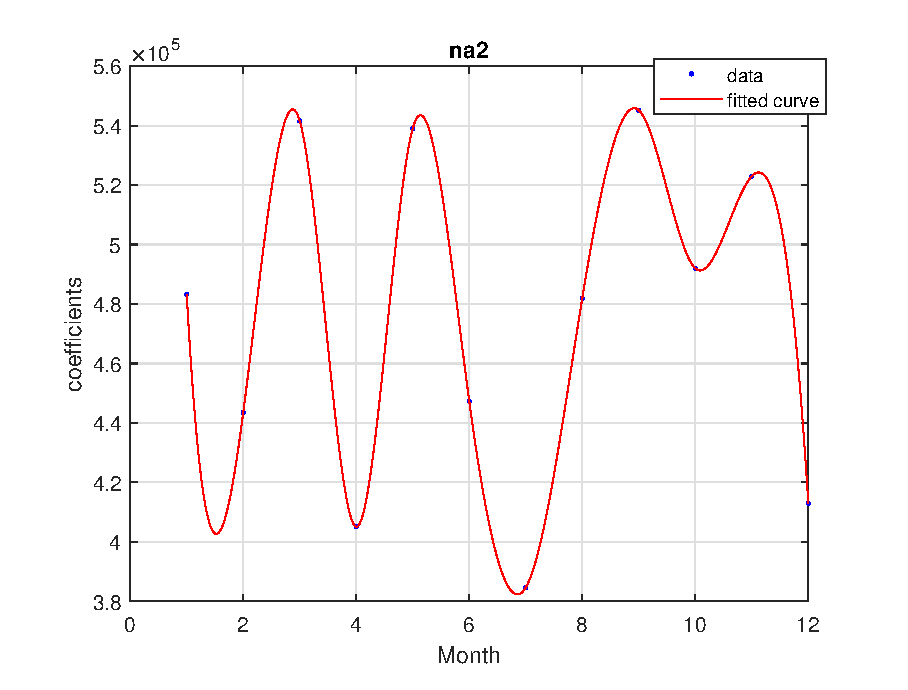
\includegraphics[width=.7\linewidth]{coeffna2.eps}
  \caption{coefficient $n_{a_{2}}$}
  \label{fig:coeffna2}
\end{subfigure}%
\begin{subfigure}{.5\textwidth}
  \centering
  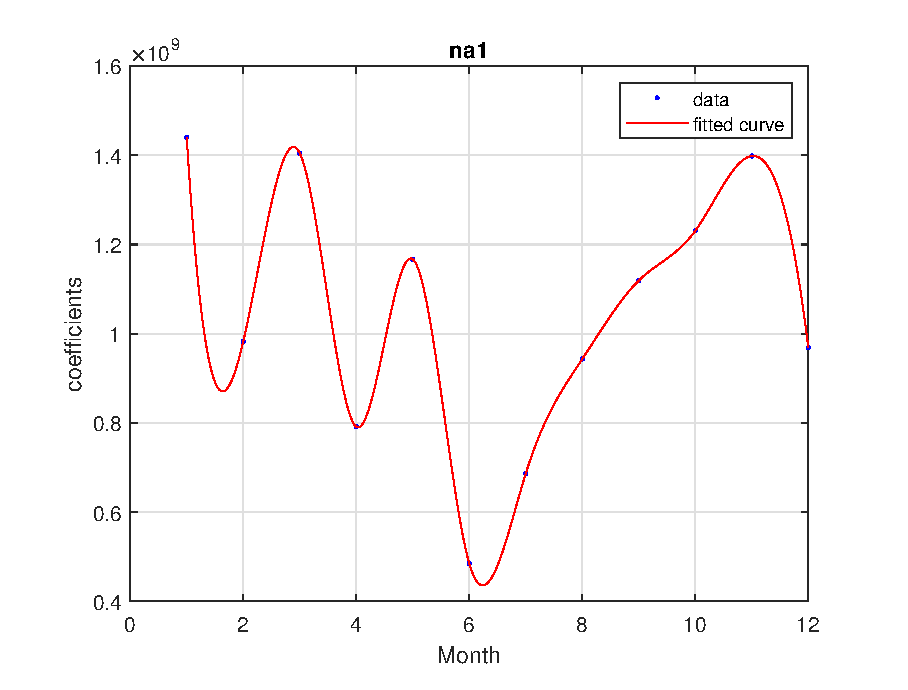
\includegraphics[width=.7\linewidth]{coeffna1.eps}
  \caption{coefficient $n_{a_{1}}$}
  \label{fig:coeffna1}
\end{subfigure}
\begin{subfigure}{.5\textwidth}
  \centering
  \includegraphics[width=.7\linewidth]{coeffnb1.eps}
  \caption{coefficient $n_{b_{1}}$}
  \label{fig:coeffnb1}
\end{subfigure}%
\begin{subfigure}{.5\textwidth}
  \centering
  \includegraphics[width=.7\linewidth]{coeffnb0.eps}
  \caption{coefficient $n_{b_{0}}$}
  \label{fig:coeffnb0}
\end{subfigure}
\caption{coefficient parameterization}
\label{fig:fitcurves}
\end{figure}


\noindent
The next step is to compare the results obtained by the Least square estimation and the one obtained by parameterization of the coefficients of the Least square estimation.Figure\ref{fig:valparG2} shows the results obtained for the month of December.We can see that the parameterization of the coefficient yields good results.

\begin{figure}[H]
    \includegraphics[width=\textwidth]{val_par_G2.png}
    \centering
    \caption{parameterization coefficient month December}
    \label{fig:valparG2}
\end{figure}

\subsection{Simultaneous identification of G1 and G2}

\newpage
\section{Conclusion}

\end{document}
